\documentclass[11pt,reqno]{amsart}

\usepackage[utf8]{inputenc}
\usepackage[T1]{fontenc}
\usepackage{lmodern}
\usepackage{amsmath,amssymb,amsfonts,amsthm,mathtools}
\usepackage{booktabs,array,multirow}
\usepackage{graphicx}
\usepackage{enumitem}
\usepackage[margin=1.0in]{geometry}
\usepackage{microtype}
\usepackage{xcolor}
\definecolor{linkblue}{rgb}{0.0,0.2,0.6}
\usepackage[colorlinks=true,linkcolor=linkblue,citecolor=linkblue,urlcolor=linkblue]{hyperref}

\newtheorem{theorem}{Theorem}[section]
\newtheorem{proposition}[theorem]{Proposition}
\newtheorem{lemma}[theorem]{Lemma}
\newtheorem{corollary}[theorem]{Corollary}
\theoremstyle{definition}
\newtheorem{definition}[theorem]{Definition}
\theoremstyle{remark}
\newtheorem{remark}[theorem]{Remark}

\numberwithin{equation}{section}
\allowdisplaybreaks

\newcommand{\R}{\mathbb{R}}
\newcommand{\C}{\mathbb{C}}
\newcommand{\N}{\mathbb{N}}
\newcommand{\Z}{\mathbb{Z}}
\newcommand{\dd}{\mathrm{d}}
\newcommand{\ee}{\mathrm{e}}
\newcommand{\ii}{\mathrm{i}}
\newcommand{\Rea}{\mathrm{Re}}
\newcommand{\Ima}{\mathrm{Im}}
\newcommand{\Tr}{\mathrm{Tr}}
\newcommand{\sinch}{\mathrm{sinc}_{\mathrm{hyp}}}
\newcommand{\fac}{\mathclose{\mathchar"0021}}

\title[Sieved Mirror Kernel and Prime-Gauge Purity]{The Sieved Mirror Kernel $\Phi_X(u)$, the Zero-Free Exponential Prime-Gauge Factor $\mathcal{E}_X(z)$, and Quadratic Prime-Power Purity on $(X, X^2]$ for Riemann's $\Xi$-Function}

\author{Thijs Missiaen}
\address{Independent Researcher, Belgium}
\email{thijs.missiaen@gmail.com}
\thanks{ORCID: \href{https://orcid.org/0009-0007-3678-0810}{0009-0007-3678-0810}}

\subjclass[2020]{Primary 11M06, 11N36; Secondary 30D15, 41A60}
\keywords{Riemann $\Xi$-function, transverse Wronskian, sieved mirror kernel, Selberg--Conrey mollifier, exponential prime-gauge factor, quadratic prime-power purity, negative hyperbolic mirror weight, Sub-Selberg closure}
\dedicatory{\upshape October 25, 2026}
\date{October 25, 2026}

\begin{document}
\sloppy

\begin{abstract}
We couple the mother-wavelet decomposition $\Phi(u) = \sum_{m=1}^{\infty} m^{-1/2}\varphi_1(u + \frac{1}{2}\ln m)$ of Riemann's Jacobi theta kernel with finite-divisor Euler-product sieving for the transverse Wronskian $W(d,t) = \frac{1}{2}\partial_d|\Xi(t - \ii d)|^2$. Multiplying $\Xi(z)$ by a self-mirrored Dirichlet polynomial $\mathcal{M}_X(z) = M_X(\frac{1}{2}+\ii z)M_X(\frac{1}{2}-\ii z)$ corresponds in the $u$-domain to an even kernel $\Phi_X(u)$ preserving the holomorphic strip $|\Ima(u)| < \frac{\pi}{8}$, whereas replacing $M_X(s)$ by the entire, zero-free exponential prime-gauge factor $E_X(s) = \exp(-\sum_{n=2}^{\lfloor X\rfloor} \frac{\Lambda(n)}{\ln n}n^{-s})$ eliminates parasitic mollifier zeros and establishes quadratic prime-power purity $b_N^{\mathcal{E}}(X) \equiv \frac{\Lambda(N)}{\ln N}$ across $\lfloor X\rfloor < N < (\lfloor X\rfloor + 1)^2$. Furthermore, we derive the negative hyperbolic mirror weight $w_n^*(d_0) = -(n^{2d_0}-1)^{-1}$ that annihilates prime-power oscillations on $d = d_0$ with zero waterbed tail for $n > X$, prove power-law $L^2$ damping $\frac{X^{-2d}}{2d\ln X}$ and Sub-Selberg closure $\theta_{\mathcal{E}}^{\mathrm{sq}}(d,t) < \frac{1}{2}$, and establish the finite-divisor identity on $[1, N(t)]$ alongside the outer factorization of $\mathcal{E}_{X,\kappa}(z)$.
\end{abstract}

\maketitle

\section{Introduction and Main Results}\label{sec:intro}

A foundational technique in the analytic theory of the Riemann zeta function $\zeta(s)$ is the attenuation of Dirichlet-series fluctuations by finite-divisor mollifiers $M_X(s) = \sum_{k \le X} c_k k^{-s}$ approximating $\zeta(s)^{-1} = \sum_{k=1}^{\infty} \mu(k)k^{-s}$, pioneered by Bohr and Landau, developed by Selberg~\cite{selberg1942}, and refined via differential calculus by Levinson~\cite{levinson1974} and Conrey~\cite{conrey1989}. When applied to the transverse Wronskian $W(d,t) := \frac{1}{2}\partial_d|\Xi(t - \ii d)|^2 = R(d,t)I_t(d,t) - I(d,t)R_t(d,t)$ of Riemann's completed function $\Xi(z) := \xi(\frac{1}{2}+\ii z) = R(d,t) + \ii\,I(d,t)$ ($z = t - \ii d$, $s = \frac{1}{2} + d + \ii t$)~\cite{riemann1859,speiser1934,hinkkanen1997,lagarias1999} or to de~Branges Hilbert-space positivity criteria~\cite{conreyli2000,csordas1986}, classical polynomial mollifiers face four structural obstacles:
\begin{enumerate}[label=\textup{(\arabic*)},leftmargin=2.2em]
\item \textit{Parasitic zeros and logarithmic-derivative waterbed tails.} Because a finite Dirichlet polynomial $M_X(s)$ possesses zeros of its own in $\C$, its logarithmic derivative $M_X'(s)/M_X(s)$ places $M_X(s)$ in the denominator, generating an infinite Dirichlet convolution tail for $n > X$ and potential small-denominator spikes.
\item \textit{Logarithmic versus power-law sieving.} Under smooth polynomial weights $c_k = \mu(k)P(\frac{\ln(X/k)}{\ln X})$ with $P(x) \sim x^r$, low harmonic shells $2 \le N \le X$ are only suppressed logarithmically by $(\ln X)^{-r}$ rather than annihilated identically, while for $N > X$ the sieved coefficients $b_N = \sum_{k \mid N,\, k \le X} c_k$ can suffer divisor-bound inflation $|b_N| \le d(N)$.
\item \textit{Conjugate mirror inflation off the critical line.} To preserve real positivity on the critical line $d = 0$, a multiplier must take the self-mirrored form $\mathcal{M}_X(z) = M_X(\frac{1}{2}+\ii z)M_X(\frac{1}{2}-\ii z)$. At $z = t - \ii d$ ($d > 0$), the conjugate factor $M_X(\frac{1}{2}-d-\ii t)$ evaluates at $\sigma_{\mathrm{conj}} = \frac{1}{2} - d < \frac{1}{2}$, where individual Dirichlet modes grow as $n^{-(1/2-d)} = n^{-1/2}n^{+d}$.
\item \textit{The Selberg barrier $\theta = \frac{1}{2}$.} Covering all active modes $1 \le n \le N(t) := \lfloor\sqrt{t/2\pi}\rfloor$ of the Riemann--Siegel main sum~\cite{siegel1932,gabcke1979} by a linear sieve requires $X \ge N(t)$ ($\theta := \frac{\ln X}{\ln(t/2\pi)} \ge \frac{1}{2}$).
\end{enumerate}

In Paper~V of this series~\cite{missiaen2026paper5}, following the Wigner phase-space~\cite{wigner1932,hudson1974}, parity-reduced Wronskian, Chladni chamber, and de~Branges--Jensen frameworks of Papers~I--IV~\cite{missiaen2026paper1,missiaen2026paper2,missiaen2026paper3,missiaen2026paper4}, we proved that every mode $\phi_m(u)$ of the Jacobi--Riemann kernel $\Phi(u) = \sum_{m=1}^{\infty} \phi_m(u)$~\cite{jacobi1829,polya1926,titchmarsh1986} is an exact logarithmic translation $\phi_m(u) = m^{-1/2}\varphi_1(u + \frac{1}{2}\ln m)$ of a single universal mother wavelet $\varphi_1(w) = (2\pi^2\ee^{9w} - 3\pi\ee^{5w})\exp(-\pi\ee^{4w})$. In the present paper (Paper~VI), we resolve all four mollifier obstacles by introducing the \emph{Sieved Mirror Kernel} $\Phi_X(u)$ in the $u$-domain and the entire, zero-free \emph{Exponential Prime-Gauge Factor} $\mathcal{E}_X(z)$. Our main results are consolidated in the following theorem.

\begin{theorem}[Sieved Mirror Kernel, Zero-Free Prime-Gauge Purity, and Sub-Selberg Closure]\label{thm:main}
Let $s = \frac{1}{2} + d + \ii t$ and $z = t - \ii d$ with $d \ge 0$ and $t > 0$, let $N(t) := \lfloor\sqrt{t/2\pi}\rfloor$ and $L := \ln(t/2\pi)$, and let $\Phi(u) = \sum_{m=1}^{\infty} m^{-1/2}\varphi_1(u + \frac{1}{2}\ln m)$. Then the following four structural laws hold:
\begin{enumerate}[label=\textup{(\roman*)},leftmargin=2.2em]
\item \textbf{Sieved Mirror Kernel $\Phi_X(u)$, Strip Preservation $|\Ima(u)| < \frac{\pi}{8}$, and Schur-Optimal Filter $P_{\mathrm{opt}}(x)$.} For any finite real Dirichlet polynomial $M_X(s) = \sum_{k=1}^{\lfloor X\rfloor} c_k k^{-s}$ with $c_1 = 1$, the self-mirrored product $\Xi_X(z) := \Xi(z)\mathcal{M}_X(z)$ with $\mathcal{M}_X(z) := M_X(\frac{1}{2}+\ii z)M_X(\frac{1}{2}-\ii z)$ preserves all zeros of $\Xi(z)$ ($\mathcal{Z}(\Xi) \subseteq \mathcal{Z}(\Xi_X)$), preserves critical-line mirror symmetry ($I_X(0,t) \equiv 0$, $\partial_d R_X(0,t) \equiv 0$, $\frac{1}{2}\partial_d|\Xi_X(t-\ii d)|^2 = W_X(d,t)$), and admits the integral representation $\Xi_X(z) = 8\int_0^{\infty} \Phi_X(u)\cos(2zu)\,\dd u$, where the even \emph{Sieved Mirror Kernel}
\begin{equation}\label{eq:intro_phi_X}
\Phi_X(u) := \sum_{j,k \le X} \frac{c_j c_k}{2\sqrt{jk}}\left[\Phi\!\left(u + \frac{1}{2}\ln\frac{j}{k}\right) + \Phi\!\left(u - \frac{1}{2}\ln\frac{j}{k}\right)\right]
\end{equation}
is holomorphic throughout the full strip $|\Ima(u)| < \frac{\pi}{8}$. Under the forward operator $\mathcal{T}_X[\Phi](u) = \sum_{N=1}^{\infty} \frac{b_N}{\sqrt{N}}\varphi_1(u + \frac{1}{2}\ln N)$ with $b_N = \sum_{k \mid N,\, k \le X} c_k$, the mother wavelet $N = 1$ remains intact ($b_1 \equiv 1$). Within the cubic Conrey--Selberg family $P(x) = x + a_2 x(1-x) + a_3 x(1-x)^2$, the unique $3 \times 3$ Schur-complement minimizer $(a_2^*, a_3^*) = (+0.81746499, +2.13817017)$ reduces quadratic cross-term energy $\mathbf{a}^T\mathbf{Q}\mathbf{a}$ by a factor of $31.4\times$ relative to Conrey's cubic filter $P_3(x)$.
\item \textbf{Zero-Free Exponential Prime-Gauge Factor $\mathcal{E}_X(z)$, Quadratic Purity on $(X, X^2]$, and Negative Hyperbolic Mirror Weight $w_n^*(d_0)$.} The exponential prime-gauge factor $E_X(s) := \exp(-\sum_{n=2}^{\lfloor X\rfloor} \frac{\Lambda(n)}{\ln n}n^{-s})$ and $\mathcal{E}_X(z) := E_X(\frac{1}{2}+\ii z)E_X(\frac{1}{2}-\ii z)$ are entire and zero-free on $\C$, so $\mathcal{Z}(\Xi_{\mathcal{E}_X}) = \mathcal{Z}(\Xi)$ bijectively. In $\zeta(s)E_X(s) = \sum_{N=1}^{\infty} b_N^{\mathcal{E}}(X)N^{-s}$, the coefficients satisfy $b_1^{\mathcal{E}}(X) = 1$, $b_N^{\mathcal{E}}(X) = 0$ for all $2 \le N \le \lfloor X\rfloor$, strict multiplicativity, universal bounds $0 \le b_N^{\mathcal{E}}(X_2) \le b_N^{\mathcal{E}}(X_1) \le 1$ ($X_2 \ge X_1$), and \emph{Quadratic Prime-Power Purity}:
\begin{equation}\label{eq:intro_quad_purity}
b_N^{\mathcal{E}}(X) \equiv \frac{\Lambda(N)}{\ln N} \qquad \text{for all } \lfloor X\rfloor < N < (\lfloor X\rfloor + 1)^2,
\end{equation}
so every composite integer with $\ge 2$ distinct prime factors in $(X, X^2]$ vanishes identically. Moreover, in the weighted gauge $\mathcal{E}_{X,\mathbf{w}}(z)$, the negative hyperbolic mirror weight $w_n^*(d_0) := -(n^{2d_0}-1)^{-1} < 0$ annihilates the effective prime-power amplitude $C_n(d_0, w_n^*(d_0)) \equiv 0$ for all $2 \le n \le \lfloor X\rfloor$ on $d = d_0$ while introducing zero terms for $n > X$ ($0\%$ waterbed tail).
\item \textbf{Power-Law $L^2$ Damping $\frac{X^{-2d}}{2d\ln X}$ and Universal Sub-Selberg Closure $\theta_{\mathcal{E}}^{\mathrm{sq}}(d,t) < \frac{1}{2}$.} For any sieve cutoff $X \in [\lfloor\sqrt{N(t)}\rfloor, N(t)]$ ($\theta = \frac{\ln X}{L} \in [\frac{1}{4}, \frac{1}{2}]$), the entire Riemann--Siegel main sum $1 \le n \le N(t) < (\lfloor X\rfloor + 1)^2$ lies inside the quadratic purity window~\eqref{eq:intro_quad_purity}, replacing logarithmic $(\ln X)^{-2r}$ decay by the power-law decay
\begin{equation}\label{eq:intro_power_law}
\mathcal{E}_{\mathrm{diag}}^{\mathcal{E},\mathrm{fwd}}(d,t;X) := \sum_{\lfloor X\rfloor < n \le N(t)} \left(\frac{\Lambda(n)}{\ln n}\right)^2 n^{-(1+2d)} \sim \frac{X^{-2d} - N(t)^{-2d}}{2d\,\ln X} < \frac{X^{-2d}}{2d\,\ln X} \longrightarrow 0,
\end{equation}
and monotonicity together with $Y^{\mathcal{E}}(d,t;N(t)) = 0$ implies $X_{\mathrm{krit}}^{\mathcal{E},\mathrm{sq}}(d,t) < N(t)$ ($\theta_{\mathcal{E}}^{\mathrm{sq}}(d,t) < \frac{1}{2}$) for all $d \in (0, \frac{1}{2}]$ and all $t \ge 8\pi$ ($N(t) \ge 2$, with $\theta_{\mathcal{E}}^{\mathrm{sq}}(d,t) = 0 < \frac{1}{2}$ on $2\pi < t < 8\pi$).
\item \textbf{Exact Finite-Divisor Identity, Composite-Gap Tail Barrier, and Shifted Outer Factorization.} The finite truncation $M_{X,N(t)}^{\mathcal{E}}(s) := \sum_{k=1}^{N(t)} c_k^{\mathcal{E}}(X)k^{-s}$ generates the exact same coefficients $b_n^{\mathcal{E}}(X)$ on $1 \le n \le N(t)$ as the infinite series $E_X(s)$, while for $n \ge N(t)+1$, the bound $0 \le b_n^{\mathcal{E}}(X) \le 1$ prevents tail inflation and composite gaps $N(t)+1 \le n < q_{\mathrm{next}}(X,t)$ deepen the Gaussian saddle-point barrier by $\exp(-\pi(q_{\mathrm{next}}^2 - (N(t)+1)^2)\allowbreak\cos 4\eta^*)$. Finally, for any $\kappa \ge 0$, the shifted self-mirrored gauge $\mathcal{E}_{X,\kappa}(z) := E_X(\frac{1}{2}+\kappa+\ii z)\allowbreak E_X(\frac{1}{2}+\kappa-\ii z)$ satisfies the exact outer factorization
\begin{equation}\label{eq:intro_outer_fact}
\bigl|\Xi_{\mathcal{E}_{X,\kappa}}(t - \ii d)\bigr|^2 \equiv \bigl|E_X(\tfrac{1}{2} + \kappa - d - \ii t)\bigr|^2 \cdot \bigl|\Xi(t - \ii d)\,E_X(\tfrac{1}{2} + \kappa + d + \ii t)\bigr|^2,
\end{equation}
eliminating conjugate $n^{+d}$ growth whenever $\kappa \ge d$.
\end{enumerate}
\end{theorem}

The canonical quantitative constants governing Theorem~\ref{thm:main} are given explicitly by
\begin{equation}\label{eq:canonical_constants}
\begin{aligned}
a_2^* &= +0.81746499\dots, & a_3^* &= +2.13817017\dots, \\
\mathcal{E}_{\mathrm{quad}}(\mathbf{a}^*) &= 2.48425572 \times 10^{-4}, & \Delta_{\mathrm{gap}}(10^8) &= -64{,}798.48\;\mathrm{dex}, \\
N_{\mathrm{comp,min}}(10) &= 11 \times 13 = 143, & N_{\mathrm{comp,min}}(50) &= 53 \times 59 = 3127.
\end{aligned}
\end{equation}

\subsection{Proof overview}\label{subsec:proof_overview}

The proof of Theorem~\ref{thm:main} is organized around three quantitative and structural ingredients:
\begin{enumerate}[label=\textup{(\arabic*)},leftmargin=2.2em]
\item \textit{Horizontal Cauchy translation in $|\Ima(u)| < \frac{\pi}{8}$ and $3\times 3$ Schur-complement minimization (Section~\ref{sec:sieved_mirror}).} Expanding $\mathcal{M}_X(z)$ as a finite cosine series $\sum_{j,k\le X}\frac{c_j c_k}{\sqrt{jk}}\cos(z\ln\frac{j}{k})$, we combine $\cos(2zu)\cos(z\ln\frac{j}{k})$ with the double-exponential decay $|\Phi(u)| = \mathcal{O}(\exp(-\pi\ee^{4|\Rea(u)|}\cos(4\Ima u)))$ to shift the contour horizontally by purely real offsets $\pm\frac{1}{2}\ln\frac{j}{k}$, preserving the full analyticity strip $|\Ima(u)| < \frac{\pi}{8}$. We then project the off-diagonal cross-term gradient onto the three-dimensional Conrey polynomial basis $\{\phi_1, \phi_2, \phi_3\}$ and solve the $2 \times 2$ Schur-complement normal equations for $(a_2^*, a_3^*)$.
\item \textit{Logarithmic-derivative generating functions and negative hyperbolic mirror cancellation (Sections~\ref{sec:prime_gauge} and~\ref{sec:power_law}).} Using $\ln\zeta(s) + \ln E_X(s) = \sum_{n > \lfloor X\rfloor}\frac{\Lambda(n)}{\ln n}n^{-s}$ for $\Rea(s) > 1$, we derive the positive tail recursion $b_N^{\mathcal{E}}(X)\ln N = \sum_{n \mid N,\, n > X} b_{N/n}^{\mathcal{E}}(X)\Lambda(n)$. Whenever $\lfloor X\rfloor < N < (\lfloor X\rfloor + 1)^2$, any divisor $n > X$ of $N$ has quotient $N/n \le \lfloor X\rfloor$, forcing $N/n = 1$ and $b_N^{\mathcal{E}}(X) = \frac{\Lambda(N)}{\ln N}$. For $X \ge \lfloor\sqrt{N(t)}\rfloor$, this quadratic purity window covers the entire Riemann--Siegel horizon $[1, N(t)]$, yielding the power-law $L^2$ bound~\eqref{eq:intro_power_law} and universal Sub-Selberg closure $\theta_{\mathcal{E}}^{\mathrm{sq}}(d,t) < \frac{1}{2}$ by partial summation over primes. In the normalized Wronskian $\Rea(\xi_{\mathcal{E}_{X,\mathbf{w}}}'/\xi_{\mathcal{E}_{X,\mathbf{w}}})$, equating the forward term $(1-w_n)n^{-(1/2+d_0)}$ against the conjugate mirror term $w_n n^{-(1/2-d_0)}$ uniquely determines $w_n^*(d_0) = -(n^{2d_0}-1)^{-1} < 0$.
\item \textit{Divisor locality on $[1, N(t)]$ and shifted outer modulus factorization (Section~\ref{sec:finite_divisor_shifted}).} Because $k \mid n \implies k \le n$, truncating $E_X(s)$ at $k = N(t)$ leaves $b_n^{\mathcal{E}}(X)$ invariant on $1 \le n \le N(t)$, while $0 \le b_n^{\mathcal{E}}(X) \le 1$ and composite gaps beyond $N(t)$ suppress the evanescent saddle-point tail. Finally, evaluating $\mathcal{E}_{X,\kappa}(z)$ at $z = t - \ii d$ separates the conjugate factor $|E_X(\frac{1}{2}+\kappa-d-\ii t)|^2 > 0$ as a scalar outer multiplier~\eqref{eq:intro_outer_fact} with exponent $\sigma_{\mathrm{conj}} = \frac{1}{2} + \kappa - d \ge \frac{1}{2}$ whenever $\kappa \ge d$.
\end{enumerate}

\subsection{Notation and conventions}\label{subsec:notation}

Consistent with Papers~I--V~\cite{missiaen2026paper1,missiaen2026paper5}, we set $s = \sigma + \ii t = \frac{1}{2} + d + \ii t$ and $z = -\ii(s - \frac{1}{2}) = t - \ii d$, with completed zeta function $\xi(s) = \frac{1}{2}s(s-1)\pi^{-s/2}\Gamma(s/2)\zeta(s)$ and $\Xi(z) := \xi(\frac{1}{2}+\ii z)$. In the canonical Mellin--Jacobi variable $x = \ee^{4u}$, $\Xi(z)$ is given by
\begin{equation}\label{eq:canonical_xi_int}
\Xi(z) = 4\int_{-\infty}^{\infty} \Phi(u)\cos(2zu)\,\dd u = 8\int_0^{\infty} \Phi(u)\cos(2zu)\,\dd u, \qquad \Phi(u) := \sum_{m=1}^{\infty} \phi_m(u),
\end{equation}
where $\phi_m(u) = (2\pi^2 m^4\ee^{9u} - 3\pi m^2\ee^{5u})\exp(-\pi m^2\ee^{4u}) = m^{-1/2}\varphi_1(u + \frac{1}{2}\ln m)$. If one rescales the integration variable to $\tilde{u} = 2u$ with $\widetilde{\Phi}(\tilde{u}) := 2\Phi(\tilde{u}/2)$, then~\eqref{eq:canonical_xi_int} takes the single-frequency form $\Xi(z) = 2\int_0^{\infty} \widetilde{\Phi}(\tilde{u})\cos(\tilde{u}z)\,\dd\tilde{u}$; throughout this paper we retain the canonical coordinate $u$ of~\eqref{eq:canonical_xi_int} so that the logarithmic shift in $\phi_m(u)$ and $\Phi_X(u)$ is $\frac{1}{2}\ln m$ and the holomorphic strip is $|\Ima(u)| < \frac{\pi}{8}$.

We maintain a strict notational distinction between the four multiplier families studied in this paper:
\begin{enumerate}[label=\textup{(\alph*)},leftmargin=2.2em]
\item $M_X(s) := \sum_{k=1}^{\lfloor X\rfloor} c_k k^{-s}$ denotes a finite polynomial Dirichlet mollifier, and $\mathcal{M}_X(z) := M_X(\frac{1}{2}+\ii z)M_X(\frac{1}{2}-\ii z)$ denotes its self-mirrored counterpart;
\item $E_X(s) := \exp(-\sum_{n=2}^{\lfloor X\rfloor} \frac{\Lambda(n)}{\ln n}n^{-s}) = \sum_{k=1}^{\infty} c_k^{\mathcal{E}}(X)k^{-s}$ denotes the unweighted exponential prime-gauge factor, and $\mathcal{E}_X(z) := E_X(\frac{1}{2}+\ii z)E_X(\frac{1}{2}-\ii z)$ denotes its self-mirrored product;
\item $E_{X,\mathbf{w}}(s) := \exp(-\sum_{n=2}^{\lfloor X\rfloor} w_n\frac{\Lambda(n)}{\ln n}n^{-s})$ and $\mathcal{E}_{X,\mathbf{w}}(z) := E_{X,\mathbf{w}}(\frac{1}{2}+\ii z)E_{X,\mathbf{w}}(\frac{1}{2}-\ii z)$ denote the weighted exponential prime-gauge factors with real weights $\mathbf{w} = (w_2, \dots, w_{\lfloor X\rfloor})$;
\item $\mathcal{E}_{X,\kappa}(z) := E_X(\frac{1}{2}+\kappa+\ii z)E_X(\frac{1}{2}+\kappa-\ii z)$ denotes the shifted self-mirrored prime-gauge factor with real shift parameter $\kappa \ge 0$.
\end{enumerate}
The ordinates of the non-trivial zeros of $\zeta(s)$ on the critical line are denoted by $\gamma_k$ (with $\gamma_1 = 14.13472514\dots$), whereas Euler's constant is denoted by $\gamma_{\mathrm{E}} = \gamma_0^{\mathrm{St}}$ and the Stieltjes constants~\cite{stieltjes1885} by $\gamma_k^{\mathrm{St}}$ ($k \ge 1$). Implied constants in $\mathcal{O}(\cdot)$ and $\ll$ are absolute unless subscripts indicate otherwise.

\section{The Sieved Mirror Kernel $\Phi_X(u)$, Holomorphic Strip Preservation $|\Ima(u)| < \frac{\pi}{8}$, and $3\times 3$ Schur-Complement Optimization $P_{\mathrm{opt}}(x)$}\label{sec:sieved_mirror}

Let $X > 1$ be a finite sieve cutoff and let $P : [0,1] \to \R$ be a smooth filter function satisfying the boundary conditions $P(0) = 0$ and $P(1) = 1$. Define the finite Dirichlet polynomial
\begin{equation}\label{eq:MX_def}
M_X(s) := \sum_{k=1}^{\lfloor X\rfloor} \frac{c_k}{k^s}, \qquad c_k := \mu(k)\,P\!\left(\frac{\ln(X/k)}{\ln X}\right) \in \R \qquad (c_1 = \mu(1)P(1) = 1),
\end{equation}
and the self-mirrored multiplier $\mathcal{M}_X(z) := M_X(\frac{1}{2}+\ii z)M_X(\frac{1}{2}-\ii z)$ with $\Xi_X(z) := \Xi(z)\mathcal{M}_X(z)$.

\begin{lemma}[Trigonometric Cosine Expansion of $\mathcal{M}_X(z)$]\label{lem:cosine_expansion}
For all $z = t - \ii d \in \C$, the self-mirrored multiplier $\mathcal{M}_X(z)$ admits the finite cosine expansion
\begin{equation}\label{eq:Mcal_cosine}
\mathcal{M}_X(z) = \sum_{j,k \le X} \frac{c_j c_k}{\sqrt{jk}}\cos\!\left(z\ln\frac{j}{k}\right) = \sum_{k \le X} \frac{c_k^2}{k} + 2\sum_{1 \le j < k \le X} \frac{c_j c_k}{\sqrt{jk}}\cos\!\left(z\ln\frac{k}{j}\right).
\end{equation}
\end{lemma}

\begin{proof}
Expanding the finite product gives
\[
\mathcal{M}_X(z) = \sum_{j,k \le X} c_j c_k\, j^{-(1/2+\ii z)}k^{-(1/2-\ii z)} = \sum_{j,k \le X} \frac{c_j c_k}{\sqrt{jk}}\exp\!\left(-\ii z\ln\frac{j}{k}\right).
\]
Since the weight $\frac{c_j c_k}{\sqrt{jk}}$ is invariant under index exchange $j \leftrightarrow k$ whereas $\ln(k/j) = -\ln(j/k)$ reverses sign, symmetrizing each $(j,k)$ and $(k,j)$ pair replaces $\exp(-\ii z\ln\frac{j}{k})$ by $\frac{1}{2}\ee^{-\ii z\ln(j/k)} +\allowbreak \frac{1}{2}\ee^{+\ii z\ln(j/k)} =\allowbreak \cos(z\ln\frac{j}{k})$.
\end{proof}

Before shifting integration contours in the $u$-domain, we record the analyticity and double-exponential decay of the Jacobi--Riemann kernel $\Phi(u)$ in horizontal strips. As established in Paper~I~\cite{missiaen2026paper1}, for $u = \xi + \ii\eta$ with $\xi \in \R$ and $|\eta| < \frac{\pi}{8}$, we have $\Rea(\pi m^2 \ee^{4u}) = \pi m^2 \ee^{4\xi}\cos(4\eta) > 0$. By the functional equation of the Jacobi theta function $\theta(x) = \sum_{n \in \Z} \ee^{-\pi n^2 x} = x^{-1/2}\theta(x^{-1})$ for $\Rea(x) > 0$, $\Phi(-u) = \Phi(u)$ is holomorphic throughout the strip $\mathcal{S}_{\pi/8} := \{u \in \C : |\Ima(u)| < \frac{\pi}{8}\}$ and satisfies the uniform double-exponential bound
\begin{equation}\label{eq:phi_strip_decay}
|\Phi(\xi + \ii\eta)| \ll \ee^{9|\xi|}\exp\!\left(-\pi\ee^{4|\xi|}\cos(4\eta)\right) \qquad (|\xi| \to \infty,\; |\eta| \le \eta_0 < \tfrac{\pi}{8}).
\end{equation}
This rapid decay justifies all contour translations and interchanges of summation and integration in the following theorem.

\begin{theorem}[Sieved Mirror Kernel and Mother-Wavelet Shell Annihilation]\label{thm:sieved_mirror_kernel}
Let $\mathcal{M}_X(z)$ be defined by~\eqref{eq:Mcal_cosine} and $\Xi_X(z) := \Xi(z)\mathcal{M}_X(z) = R_X(d,t) + \ii\,I_X(d,t)$ for $z = t - \ii d$. Then:
\begin{enumerate}[label=\textup{(\alph*)},leftmargin=2.2em]
\item \textbf{Zero inclusion and critical-line mirror symmetry.} $\mathcal{M}_X(z)$ is an entire function on $\C$, so $\mathcal{Z}(\Xi) \subseteq \mathcal{Z}(\Xi_X)$, and at every critical-line zero $\gamma_k \in \R$ of $\Xi(z)$ the parity-reduced Wronskian $\widetilde{W}_X(d,t) := W_X(d,t)/d$ satisfies
\begin{equation}\label{eq:Wtilde_zero_slope}
\widetilde{W}_X(0,\gamma_k) = \bigl(\Xi'(\gamma_k)\bigr)^2\,\bigl|M_X(\tfrac{1}{2} + \ii\gamma_k)\bigr|^4 \ge 0.
\end{equation}
Moreover, $\Xi_X(\bar{z}) = \overline{\Xi_X(z)}$, so $R_X(-d,t) = R_X(d,t)$, $I_X(-d,t) = -I_X(d,t)$, $I_X(0,t) \equiv 0$, $\partial_d R_X(0,t) \equiv 0$, $\Delta R_X = \Delta I_X \equiv 0$, and $\frac{1}{2}\partial_d|\Xi_X(t-\ii d)|^2 = W_X(d,t) = R_X\partial_t I_X - I_X\partial_t R_X$.
\item \textbf{Sieved Mirror Kernel $\Phi_X(u)$ and holomorphic strip preservation.} For all $z \in \C$, $\Xi_X(z)$ is the Fourier cosine transform
\begin{equation}\label{eq:XiX_fourier}
\Xi_X(z) = 4\int_{-\infty}^{\infty} \Phi_X(u)\cos(2zu)\,\dd u = 8\int_0^{\infty} \Phi_X(u)\cos(2zu)\,\dd u = 2\int_0^{\infty} \widetilde{\Phi}_X(\tilde{u})\cos(\tilde{u}z)\,\dd\tilde{u},
\end{equation}
where $\widetilde{\Phi}_X(\tilde{u}) := 2\Phi_X(\tilde{u}/2)$ and the \emph{Sieved Mirror Kernel} $\Phi_X(u)$ defined by~\eqref{eq:intro_phi_X} is even ($\Phi_X(-u) = \Phi_X(u)$) and preserves the full holomorphic strip $|\Ima(u)| < \frac{\pi}{8}$.
\item \textbf{Mother-Wavelet shell annihilation.} Under the one-sided Dirichlet shift operator $\mathcal{T}_X[\Phi](u)$, the mother-wavelet expansion of $\Phi(u)$ transforms into
\begin{equation}\label{eq:TX_mother_wavelet}
\mathcal{T}_X[\Phi](u) := \sum_{k \le X} \frac{c_k}{\sqrt{k}}\,\Phi\!\left(u + \frac{1}{2}\ln k\right) = \sum_{N=1}^{\infty} \frac{b_N}{\sqrt{N}}\,\varphi_1\!\left(u + \frac{1}{2}\ln N\right), \qquad b_N := \sum_{\substack{k \mid N \\ k \le X}} c_k,
\end{equation}
where $\zeta(s)M_X(s) = \sum_{N=1}^{\infty} b_N N^{-s}$. In particular, the mother wavelet $N = 1$ remains $100\%$ intact ($b_1 = c_1 \equiv 1$), while for $P_1(x) = x$ all composite integers $2 \le N \le X$ with $\ge 2$ distinct prime factors satisfy $b_N^{(1)} = \frac{\Lambda(N)}{\ln X} = 0$.
\end{enumerate}
\end{theorem}

\begin{proof}
(a) Each term $k^{-(1/2 \pm \ii z)} = \exp(-(1/2 \pm \ii z)\ln k)$ is entire on $\C$, so $\mathcal{M}_X(z)$ has no poles in $\C$ and $\Xi(z_0) = 0 \implies \Xi_X(z_0) = 0$. At a critical-line zero $\Xi(\gamma_k) = 0$, the product rule gives $\Xi_X'(\gamma_k) = \Xi'(\gamma_k)\mathcal{M}_X(\gamma_k) = \Xi'(\gamma_k)|M_X(\frac{1}{2}+\ii\gamma_k)|^2$, whence $\widetilde{W}_X(0,\gamma_k) = (\Xi_X'(\gamma_k))^2$ yields~\eqref{eq:Wtilde_zero_slope}. Because $c_k \in \R$, Lemma~\ref{lem:cosine_expansion} and $\cos(\bar{w}) = \overline{\cos w}$ imply $\mathcal{M}_X(\bar{z}) = \overline{\mathcal{M}_X(z)}$. Combining this with $\Xi(\bar{z}) = \overline{\Xi(z)}$ gives $\Xi_X(t + \ii d) = \overline{\Xi_X(t - \ii d)}$, which forces $R_X(-d,t) = R_X(d,t)$ and $I_X(-d,t) = -I_X(d,t)$. Holomorphicity in $z = t - \ii d$ implies $\partial_d R_X = \partial_t I_X$ and $\partial_d I_X = -\partial_t R_X$, yielding harmonicity and $\frac{1}{2}\partial_d(R_X^2 + I_X^2) = R_X\partial_t I_X - I_X\partial_t R_X = W_X(d,t)$.

(b) Multiplying $\Xi(z) = 4\int_{-\infty}^{\infty} \Phi(u)\cos(2zu)\,\dd u$ by~\eqref{eq:Mcal_cosine} and applying the trigonometric identity
\[
\cos(2zu)\cos\!\left(z\ln\frac{j}{k}\right) = \frac{1}{2}\left[\cos\!\left(2z\!\left(u - \frac{1}{2}\ln\frac{j}{k}\right)\right) + \cos\!\left(2z\!\left(u + \frac{1}{2}\ln\frac{j}{k}\right)\right)\right],
\]
the translation invariance of Lebesgue integration on $\R$ ($u \mp \frac{1}{2}\ln(j/k) \mapsto u$, justified for all $z \in \C$ by the double-exponential bound~\eqref{eq:phi_strip_decay}) yields~\eqref{eq:XiX_fourier} with $\Phi_X(u)$ given by~\eqref{eq:intro_phi_X}. Because every shift $\pm\frac{1}{2}\ln(j/k) \in \R$ is purely real, $\Ima(u \pm \frac{1}{2}\ln\frac{j}{k}) = \Ima(u)$, so the singularities of $\Phi(u \pm \frac{1}{2}\ln\frac{j}{k})$ remain on the horizontal lines $\Ima(u) = \pm\frac{\pi}{8}$. Hence $\Phi_X(u)$ is even and holomorphic throughout $|\Ima(u)| < \frac{\pi}{8}$.

(c) Substituting $\Phi(u + \frac{1}{2}\ln k) = \sum_{m=1}^{\infty} m^{-1/2}\varphi_1(u + \frac{1}{2}\ln k + \frac{1}{2}\ln m)$ into $\mathcal{T}_X[\Phi](u)$ and grouping the absolutely convergent double series (justified by~\eqref{eq:phi_strip_decay}) by the product index $N = km$ gives $\frac{1}{\sqrt{k}}\frac{1}{\sqrt{m}} = \frac{1}{\sqrt{N}}$ and $\frac{1}{2}\ln k + \frac{1}{2}\ln m = \frac{1}{2}\ln N$, proving~\eqref{eq:TX_mother_wavelet}. For $N = 1$, only $k = 1$ divides $1$, so $b_1 = c_1 = 1$. For Selberg's linear filter $P_1(x) = x = 1 - \frac{\ln k}{\ln X}$ and $2 \le N \le X$, the classical identities $\sum_{k \mid N} \mu(k) = 0$ and $-\sum_{k \mid N} \mu(k)\ln k = \Lambda(N)$ give $b_N^{(1)} = \frac{\Lambda(N)}{\ln X}$.
\end{proof}

We now show how the higher-degree polynomial coefficients of $P(x)$ can be chosen via a positive semi-definite quadratic form to minimize off-diagonal cross-term interference between the mother wavelet ($m = 1$) and the satellite shells $2 \le n \le N_{\max}$.

\begin{proposition}[Quadratic Cross-Term Form and $3\times 3$ Schur-Complement Filter $P_{\mathrm{opt}}(x)$]\label{prop:schur_filter}
Consider the cubic Conrey--Selberg filter family satisfying $P(0) = 0$ and $P(1) = 1$:
\begin{equation}\label{eq:Conrey_cubic_family}
P(x) = \phi_1(x) + a_2\,\phi_2(x) + a_3\,\phi_3(x), \qquad \phi_1(x) := x, \quad \phi_2(x) := x(1-x), \quad \phi_3(x) := x(1-x)^2,
\end{equation}
parameterized by $\mathbf{a} := (1, a_2, a_3)^T \in \{1\} \times \R^2$. Then the sieved coefficients $b_n(\mathbf{a}) = \sum_{\alpha=1}^3 a_\alpha b_n^{(\alpha)}$ are affine-linear in $(a_2, a_3)$ with $b_1(\mathbf{a}) \equiv 1$. For any compact spectral interval $[T_1, T_2]$ with active horizon $N_{\max} = N(T_2)$ and mother-wavelet cross-waveforms $\Psi_\alpha(d,t) := \sum_{n=2}^{N_{\max}} b_n^{(\alpha)} K_{1,n}(d,t)$ (where $K_{1,n}(d,t) := \frac{4}{\sqrt{n}}[L_{1,n}^+\sinh(dL_{1,n}^+)\cos(t\ln n) + (\ln n)\sinh(d\ln n)\cos(2\vartheta(t) - t\ln n)]$ with $L_{1,n}^+ := \ln(\frac{t}{2\pi n})$ is the mother-wavelet cross-kernel of Paper~V~\cite{missiaen2026paper5}), the mean-square cross-term gradient energy is the $3 \times 3$ quadratic form
\begin{equation}\label{eq:E_quad_form}
\mathcal{E}_{\mathrm{quad}}(\mathbf{a}) := \frac{1}{T_2 - T_1}\int_{T_1}^{T_2} \left(\sum_{\alpha=1}^3 a_\alpha\,\Psi_\alpha(d,t)\right)^{\!2} \dd t = \mathbf{a}^T \mathbf{Q}\,\mathbf{a}, \quad Q_{\alpha\beta} := \frac{1}{T_2 - T_1}\int_{T_1}^{T_2} \Psi_\alpha(d,t)\,\Psi_\beta(d,t)\,\dd t.
\end{equation}
Whenever the $2 \times 2$ principal block $\mathbf{Q}_{22} := (Q_{\alpha\beta})_{2 \le \alpha,\beta \le 3}$ is positive definite, $\mathcal{E}_{\mathrm{quad}}(\mathbf{a})$ possesses the unique global minimizer and Schur-complement minimum value
\begin{equation}\label{eq:schur_minimizer}
\begin{pmatrix} a_2^* \\ a_3^* \end{pmatrix} = -\mathbf{Q}_{22}^{-1}\begin{pmatrix} Q_{21} \\ Q_{31} \end{pmatrix}, \qquad \mathcal{E}_{\mathrm{quad}}(\mathbf{a}^*) = Q_{11} - \begin{pmatrix} Q_{12} & Q_{13} \end{pmatrix} \mathbf{Q}_{22}^{-1} \begin{pmatrix} Q_{21} \\ Q_{31} \end{pmatrix}.
\end{equation}
On $[T_1, T_2] = [14, 300]$ ($N_{\max} = 6$, $d = 0.20$, $X = 50$), equation~\eqref{eq:schur_minimizer} gives $(a_2^*, a_3^*) = (+0.81746499,\allowbreak +2.13817017)$ and $\mathcal{E}_{\mathrm{quad}}(\mathbf{a}^*) = 2.48425572 \times 10^{-4}$, which is $31.41\times$ smaller than Conrey's cubic filter $P_3(x)$ ($\mathbf{a} = (1,1,1)^T$, $\mathcal{E}_{\mathrm{quad}} = 7.8021 \times 10^{-3}$) and $2605.7\times$ smaller ($99.9616\%$ reduction) than Selberg's linear filter $P_1(x)$ ($\mathbf{a} = (1,0,0)^T$, $\mathcal{E}_{\mathrm{quad}} = 0.647448$).
\end{proposition}

\begin{proof}
Because $\phi_1(1) = 1$ and $\phi_2(1) = \phi_3(1) = 0$, we have $c_1^{(1)} = 1$ and $c_1^{(2)} = c_1^{(3)} = 0$, so $b_1(\mathbf{a}) = 1 + 0\cdot a_2 + 0\cdot a_3 \equiv 1$. By linearity of the finite divisor sum $b_n(\mathbf{a}) = \sum_{k \mid n,\, k \le X} \sum_{\alpha=1}^3 a_\alpha c_k^{(\alpha)}$, the cross-term gradient $\sum_{n=2}^{N_{\max}} b_n(\mathbf{a}) K_{1,n}(d,t)$ equals $\sum_{\alpha=1}^3 a_\alpha \Psi_\alpha(d,t)$, whose $L^2([T_1, T_2])$ inner product is~\eqref{eq:E_quad_form}. Writing $\mathbf{a} = (1, \tilde{\mathbf{a}})^T$ with $\tilde{\mathbf{a}} = (a_2, a_3)^T$ and $\mathbf{q}_1 = (Q_{21}, Q_{31})^T$, completion of the square gives
\[
\mathbf{a}^T\mathbf{Q}\,\mathbf{a} = Q_{11} + 2\mathbf{q}_1^T\tilde{\mathbf{a}} + \tilde{\mathbf{a}}^T\mathbf{Q}_{22}\tilde{\mathbf{a}} = \left(\tilde{\mathbf{a}} + \mathbf{Q}_{22}^{-1}\mathbf{q}_1\right)^T \mathbf{Q}_{22}\left(\tilde{\mathbf{a}} + \mathbf{Q}_{22}^{-1}\mathbf{q}_1\right) + \left(Q_{11} - \mathbf{q}_1^T\mathbf{Q}_{22}^{-1}\mathbf{q}_1\right),
\]
establishing~\eqref{eq:schur_minimizer}. The explicit Gram matrix entries and interval-arithmetic certification are detailed in Appendix~\ref{app:schur}.
\end{proof}

\begin{table}[t]
\centering
\caption{Comparison of sieved shell coefficients $b_N$ ($1 \le N \le 9$) and cross-term suppression metrics on $t \in [14, 300]$ ($d = 0.20, X = 50$), certified in \texttt{mpmath} (\texttt{mp.dps = 50}) and \texttt{mpmath.iv} (\texttt{iv.dps = 35}).}\label{tab:schur_optimization}
\scriptsize
\setlength{\tabcolsep}{3.6pt}
\begin{tabular}{@{}lcccccc@{}}
\toprule
Quantity / Metric & Unsieved & Selberg $P_1(x)$ & Conrey $P_2(x)$ & Conrey $P_3(x)$ & Schur $P_{\mathrm{opt}}(x)$ & Exp-Gauge $E_X$ \\
\midrule
Parameter pair $(a_2, a_3)$ & --- & $(0, 0)$ & $(1, 0)$ & $(1, 1)$ & $(0.8175, 2.1382)$ & Log-Euler \\
Mother Wavelet $b_1$ ($N=1$) & $+1.000000$ & $+1.000000$ & $+1.000000$ & $+1.000000$ & $+1.000000$ & $+1.000000$ \\
Prime shell $b_2$ ($N=2$) & $+1.000000$ & $+0.177184$ & $+0.031394$ & $+0.005563$ & $+0.002774$ & $0.000000$ \\
Prime shell $b_3$ ($N=3$) & $+1.000000$ & $+0.280830$ & $+0.078865$ & $+0.022148$ & $-0.005541$ & $0.000000$ \\
Prime-power shell $b_4$ ($2^2$) & $+1.000000$ & $+0.177184$ & $+0.031394$ & $+0.005563$ & $+0.002774$ & $0.000000$ \\
Prime shell $b_5$ ($N=5$) & $+1.000000$ & $+0.411408$ & $+0.169257$ & $+0.069634$ & $+0.000447$ & $0.000000$ \\
Composite shell $b_6$ ($2\cdot 3$) & $+1.000000$ & $0.000000$ & $-0.099517$ & $-0.068370$ & $-0.014754$ & $0.000000$ \\
Prime shell $b_7$ ($N=7$) & $+1.000000$ & $+0.497418$ & $+0.247425$ & $+0.123073$ & $+0.027173$ & $0.000000$ \\
Quadratic energy $\mathbf{a}^T\mathbf{Q}\mathbf{a}$ & --- & $0.647448$ & $0.054728$ & $0.007802$ & $0.000248$ & $0.000000$ \\
Full RS cross-term $\mathrm{RMS}|\partial_d\mathcal{C}_N|$ & $4.150934$ & $0.830237$ & $0.238616$ & $0.090088$ & $0.016084$ & $0.000000$ \\
Stability $\min_t(W_X/D_{\mathrm{diag}})$ & $+0.019086$ & $+0.655414$ & $+0.862846$ & $+0.943060$ & $+0.992231$ & $+1.000000$ \\
\bottomrule
\end{tabular}
\end{table}

\section{The Zero-Free Exponential Prime-Gauge Factor $\mathcal{E}_X(z)$, Quadratic Prime-Power Purity on $(X, X^2]$, and Negative Hyperbolic Mirror Annihilation $w_n^*(d_0)$}\label{sec:prime_gauge}

While the polynomial mollifier $\mathcal{M}_X(z)$ is pole-free, $M_X(s)$ can vanish in $\C$ and leaves non-zero residual prime shells $b_N \neq 0$ for $2 \le N \le X$. To eliminate both parasitic mollifier zeros and all residual shells up to $X$, we exponentiate the truncated logarithmic Euler product:
\begin{equation}\label{eq:EX_def}
E_X(s) := \exp\!\left(-\sum_{n=2}^{\lfloor X\rfloor} \frac{\Lambda(n)}{\ln n}\,n^{-s}\right) = \sum_{k=1}^{\infty} c_k^{\mathcal{E}}(X)\,k^{-s}, \qquad \mathcal{E}_X(z) := E_X\!\left(\frac{1}{2} + \ii z\right)E_X\!\left(\frac{1}{2} - \ii z\right).
\end{equation}
Because the exponent $\mathcal{P}_X(z) := -2\sum_{n=2}^{\lfloor X\rfloor} \frac{\Lambda(n)}{(\ln n)\sqrt{n}}\cos(z\ln n)$ is a finite sum of entire cosine functions, $\mathcal{E}_X(z) = \exp(\mathcal{P}_X(z))$ has \emph{zero poles and zero parasitic zeros anywhere in $\C$}, so $\Xi_{\mathcal{E}_X}(z) := \Xi(z)\mathcal{E}_X(z)$ satisfies $\mathcal{Z}(\Xi_{\mathcal{E}_X}) = \mathcal{Z}(\Xi)$ bijectively with identical multiplicities.

\begin{theorem}[Number-Theoretic Characterization of $b_N^{\mathcal{E}}(X)$ and Quadratic Prime-Power Purity Window]\label{thm:quadratic_purity}
Let $X \ge 1$ and define the sieved Dirichlet coefficients $b_N^{\mathcal{E}}(X)$ for $\Rea(s) > 1$ by
\begin{equation}\label{eq:zeta_EX_product}
\zeta(s)\,E_X(s) = \exp\!\left(\sum_{n > \lfloor X\rfloor} \frac{\Lambda(n)}{\ln n}\,n^{-s}\right) = \sum_{N=1}^{\infty} b_N^{\mathcal{E}}(X)\,N^{-s}.
\end{equation}
Then the following four arithmetic laws hold:
\begin{enumerate}[label=\textup{(\roman*)},leftmargin=2.2em]
\item \textbf{Exact M\"obius recursion and shell annihilation up to $X$.} The coefficients $c_k^{\mathcal{E}}(X)$ of $E_X(s)$ satisfy $c_1^{\mathcal{E}}(X) = 1$, $c_k^{\mathcal{E}}(X)\ln k = -\sum_{n \mid k,\, 2 \le n \le \lfloor X\rfloor} c_{k/n}^{\mathcal{E}}(X)\Lambda(n)$ for $k \ge 2$, and $c_k^{\mathcal{E}}(X) \equiv \mu(k)$ for all $1 \le k \le \lfloor X\rfloor$. Simultaneously, $b_N^{\mathcal{E}}(X)$ obeys the positive tail recursion
\begin{equation}\label{eq:bN_tail_recursion}
b_1^{\mathcal{E}}(X) = 1, \qquad b_N^{\mathcal{E}}(X)\,\ln N = \sum_{\substack{n \mid N \\ n > \lfloor X\rfloor}} b_{N/n}^{\mathcal{E}}(X)\,\Lambda(n) \qquad (N \ge 2),
\end{equation}
which implies $b_N^{\mathcal{E}}(X) = 0$ identically for all $2 \le N \le \lfloor X\rfloor$.
\item \textbf{Strict multiplicativity and unitary prime-power support.} $b_N^{\mathcal{E}}(X)$ is multiplicative: $b_{MN}^{\mathcal{E}}(X) = b_M^{\mathcal{E}}(X)b_N^{\mathcal{E}}(X)$ whenever $\gcd(M,N) = 1$. For an arbitrary integer with canonical prime factorization $N = \prod_{i=1}^r p_i^{\alpha_i}$,
\begin{equation}\label{eq:unitary_support}
b_N^{\mathcal{E}}(X) = \prod_{i=1}^r b_{p_i^{\alpha_i}}^{\mathcal{E}}(X) > 0 \iff \text{every unitary prime-power divisor } p_i^{\alpha_i} \parallel N \text{ satisfies } p_i^{\alpha_i} > X.
\end{equation}
\item \textbf{Universal $0\%$ overshoot and monotonicity in $X$.} For all $N \ge 1$ and all $X_2 \ge X_1 \ge 1$,
\begin{equation}\label{eq:universal_bounds_mono}
0 \le b_N^{\mathcal{E}}(X_2) \le b_N^{\mathcal{E}}(X_1) \le b_N^{\mathcal{E}}(1) = 1.
\end{equation}
\item \textbf{Quadratic Prime-Power Purity on $\lfloor X\rfloor < N < (\lfloor X\rfloor + 1)^2$.} Throughout the entire quadratic window $\lfloor X\rfloor < N < (\lfloor X\rfloor + 1)^2$ (and in particular on $(X, X^2]$),
\begin{equation}\label{eq:quadratic_purity_law}
b_N^{\mathcal{E}}(X) \equiv \frac{\Lambda(N)}{\ln N} = \begin{cases}
1 & \text{if } N = p \text{ is prime}, \\
1/k & \text{if } N = p^k \text{ is a higher prime power } (k \ge 2), \\
0 & \text{if } N \text{ is composite with } \ge 2 \text{ distinct prime factors}.
\end{cases}
\end{equation}
Consequently, the smallest composite integer with $\ge 2$ distinct prime factors having $b_N^{\mathcal{E}}(X) > 0$ is $N_{\mathrm{comp,min}}(X) = q_1(X)q_2(X) \ge (\lfloor X\rfloor + 1)(\lfloor X\rfloor + 2) > X^2$, where $q_1(X) < q_2(X)$ are the two smallest coprime prime powers exceeding $X$.
\end{enumerate}
\end{theorem}

\begin{proof}
(i) For $\Rea(s) > 1$, the Euler product $\zeta(s) = \prod_p (1 - p^{-s})^{-1}$ has logarithmic series $\ln\zeta(s) = \sum_{n=2}^{\infty} \frac{\Lambda(n)}{\ln n}n^{-s}$. Adding $\ln E_X(s) = -\sum_{n=2}^{\lfloor X\rfloor} \frac{\Lambda(n)}{\ln n}n^{-s}$ cancels all terms $2 \le n \le \lfloor X\rfloor$ and yields~\eqref{eq:zeta_EX_product}. Differentiating $E_X(s)$ and $\zeta(s)E_X(s)$ gives $-E_X'(s) = E_X(s)\sum_{n=2}^{\lfloor X\rfloor} \Lambda(n)n^{-s}$ and $-(\zeta E_X)'(s) = (\zeta E_X)(s)\sum_{n > \lfloor X\rfloor} \Lambda(n)n^{-s}$; equating coefficients of $k^{-s}$ and $N^{-s}$ yields the recursion for $c_k^{\mathcal{E}}(X)$ and~\eqref{eq:bN_tail_recursion}. For $1 \le k \le \lfloor X\rfloor$, every divisor $n \mid k$ satisfies $n \le k \le \lfloor X\rfloor$, so $c_k^{\mathcal{E}}(X)$ obeys the exact same recursion $\mu(k)\ln k = -\sum_{n \mid k} \mu(k/n)\Lambda(n)$ as the M\"obius function, proving $c_k^{\mathcal{E}}(X) = \mu(k)$ by induction. For $2 \le N \le \lfloor X\rfloor$, the sum in~\eqref{eq:bN_tail_recursion} is empty, so $b_N^{\mathcal{E}}(X) = 0$.

(ii) Grouping the exponent $R_{>X}(s) := \sum_{n > \lfloor X\rfloor} \frac{\Lambda(n)}{\ln n}n^{-s}$ by prime base $p$ with threshold exponent $k_p(X) := \lfloor\log_p X\rfloor + 1 = \min\{k \ge 1 : p^k > X\}$ gives the Euler-type factorization
\[
\zeta(s)\,E_X(s) = \prod_p \exp\!\left(\sum_{k = k_p(X)}^{\infty} \frac{p^{-ks}}{k}\right) = \prod_p \left(1 + \sum_{\alpha=1}^{\infty} b_{p^\alpha}^{\mathcal{E}}(X)\,p^{-\alpha s}\right).
\]
Because factors indexed by distinct primes $p$ involve coprime Dirichlet frequencies $p^{-\alpha s}$, $b_N^{\mathcal{E}}(X)$ is multiplicative. For a single prime power $p^\alpha$, the series $\sum_{k \ge k_p(X)} \frac{p^{-ks}}{k}$ starts at degree $k_p(X)$, so $b_{p^\alpha}^{\mathcal{E}}(X) = 0$ if $\alpha < k_p(X)$ (i.e., $p^\alpha \le X$) and $b_{p^\alpha}^{\mathcal{E}}(X) \ge \frac{1}{\alpha} > 0$ if $\alpha \ge k_p(X)$ (i.e., $p^\alpha > X$). Multiplicativity over $p_i^{\alpha_i} \parallel N$ immediately yields~\eqref{eq:unitary_support}.

(iii) For $X_2 \ge X_1 \ge 1$, write $R_{>X_1}(s) = R_{>X_2}(s) + \Delta(s)$ with $\Delta(s) := \sum_{\lfloor X_1\rfloor < n \le \lfloor X_2\rfloor} \frac{\Lambda(n)}{\ln n}n^{-s}$. Since both $R_{>X_2}(s)$ and $\Delta(s)$ have non-negative Dirichlet coefficients, expanding $\exp(R_{>X_1}(s)) = \exp(R_{>X_2}(s))\sum_{m=0}^{\infty} \frac{1}{m\fac}\Delta(s)^m$ shows coefficientwise that $0 \le b_N^{\mathcal{E}}(X_2) \le b_N^{\mathcal{E}}(X_1)$. Taking $X_1 = 1$ gives $\exp(R_{>1}(s)) = \zeta(s) = \sum_{N=1}^{\infty} 1\cdot N^{-s}$, so $b_N^{\mathcal{E}}(1) = 1$, establishing~\eqref{eq:universal_bounds_mono}.

(iv) Let $\lfloor X\rfloor < N < (\lfloor X\rfloor + 1)^2$. In the recursion~\eqref{eq:bN_tail_recursion}, every divisor $n \mid N$ satisfying $n \ge \lfloor X\rfloor + 1$ has complementary quotient $m := N/n < \frac{(\lfloor X\rfloor + 1)^2}{\lfloor X\rfloor + 1} = \lfloor X\rfloor + 1$, so $1 \le m \le \lfloor X\rfloor$. By part~(i), $b_m^{\mathcal{E}}(X) = 0$ for all $2 \le m \le \lfloor X\rfloor$, so only $m = 1$ ($n = N$) contributes to~\eqref{eq:bN_tail_recursion}, yielding $b_N^{\mathcal{E}}(X)\ln N = b_1^{\mathcal{E}}(X)\Lambda(N) = \Lambda(N)$ and proving~\eqref{eq:quadratic_purity_law}.
\end{proof}

We next resolve Open Problem~7 (the pointwise waterbed and mirror-inflation effect in the normalized Wronskian). Consider the weighted exponential prime-gauge factor with real weights $\mathbf{w} = (w_2, \dots, w_{\lfloor X\rfloor}) \in \R^{\lfloor X\rfloor - 1}$:
\begin{equation}\label{eq:EX_weighted_def}
E_{X,\mathbf{w}}(s) := \exp\!\left(-\sum_{n=2}^{\lfloor X\rfloor} w_n\frac{\Lambda(n)}{\ln n}n^{-s}\right), \quad \mathcal{E}_{X,\mathbf{w}}(z) := E_{X,\mathbf{w}}\!\left(\tfrac{1}{2}+\ii z\right)E_{X,\mathbf{w}}\!\left(\tfrac{1}{2}-\ii z\right) = \exp\!\bigl(\mathcal{P}_{X,\mathbf{w}}(z)\bigr),
\end{equation}
where $\mathcal{P}_{X,\mathbf{w}}(z) = -2\sum_{n=2}^{\lfloor X\rfloor} w_n\frac{\Lambda(n)}{(\ln n)\sqrt{n}}\cos(z\ln n)$, and set $\Xi_{\mathcal{E}_{X,\mathbf{w}}}(z) := \Xi(z)\mathcal{E}_{X,\mathbf{w}}(z)$.

\begin{theorem}[Exact Negative Hyperbolic Mirror Weight $w_n^*(d_0) = -(n^{2d_0}-1)^{-1}$ Without Waterbed Tail]\label{thm:hyperbolic_mirror_weight}
For all $(d,t) \in \R^2$ outside the zeros of $\Xi$, the normalized transverse Wronskian of $\Xi_{\mathcal{E}_{X,\mathbf{w}}}(z)$ equals $\Rea(\xi'(s)/\xi(s)) + \partial_d\,\Rea\,\mathcal{P}_{X,\mathbf{w}}(t - \ii d)$ and satisfies the exact additive identity
\begin{equation}\label{eq:normalized_wronskian_weighted}
\frac{W_{\mathcal{E}_{X,\mathbf{w}}}(d,t)}{\bigl|\Xi_{\mathcal{E}_{X,\mathbf{w}}}(t - \ii d)\bigr|^2} = \Rea\!\left(\frac{\xi'(s)}{\xi(s)}\right) - 2\sum_{n=2}^{\lfloor X\rfloor} w_n\frac{\Lambda(n)}{\sqrt{n}}\sinh(d\ln n)\cos(t\ln n).
\end{equation}
Combined with the Dirichlet series $-\frac{\zeta'(s)}{\zeta(s)} = \sum_{n=2}^{\infty} \Lambda(n)n^{-s}$ and the Archimedean digamma drift $\mathcal{A}(d,t) := \Rea(\frac{1}{s} + \frac{1}{s-1} - \frac{1}{2}\ln\pi + \frac{1}{2}\psi(\frac{s}{2}))$, the effective amplitude of the $n$-th prime power ($2 \le n \le \lfloor X\rfloor$) is
\begin{equation}\label{eq:Cn_effective}
C_n(d, w_n) := (1 - w_n)\,n^{-(1/2+d)} + w_n\,n^{-(1/2-d)} = n^{-(1/2+d)} + 2w_n\,n^{-1/2}\sinh(d\ln n).
\end{equation}
For any target transverse line $d_0 > 0$, choosing the \emph{negative hyperbolic mirror weight}
\begin{equation}\label{eq:w_star_boxed}
\boxed{w_n^*(d_0) := -\frac{n^{-d_0}}{n^{+d_0} - n^{-d_0}} = -\frac{1}{n^{2d_0} - 1} < 0 \qquad (\forall\, d_0 > 0,\; 2 \le n \le \lfloor X\rfloor)}
\end{equation}
annihilates $C_n(d_0, w_n^*(d_0)) \equiv 0$ identically for all $2 \le n \le \lfloor X\rfloor$ on the line $d = d_0$, while introducing \emph{zero terms for $n > X$ ($0\%$ convolution/waterbed tail)} in the logarithmic derivative:
\begin{equation}\label{eq:tail_free_cancellation}
\frac{W_{\mathcal{E}_{X,\mathbf{w}^*(d_0)}}(d_0,t)}{\bigl|\Xi_{\mathcal{E}_{X,\mathbf{w}^*(d_0)}}(t - \ii d_0)\bigr|^2} = \Rea\!\left(\frac{\xi'(\frac{1}{2}+d_0+\ii t)}{\xi(\frac{1}{2}+d_0+\ii t)}\right) + \sum_{n=2}^{\lfloor X\rfloor} \frac{\Lambda(n)}{n^{1/2+d_0}}\cos(t\ln n) \qquad (\forall\, t \in \R).
\end{equation}
\end{theorem}

\begin{proof}
Since $\frac{1}{2}\partial_d\ln|\Xi_{\mathcal{E}_{X,\mathbf{w}}}(t-\ii d)|^2 =\allowbreak W_{\mathcal{E}_{X,\mathbf{w}}}(d,t)/\allowbreak|\Xi_{\mathcal{E}_{X,\mathbf{w}}}(t-\ii d)|^2$ and $\ln|\Xi_{\mathcal{E}_{X,\mathbf{w}}}| =\allowbreak \ln|\xi(s)| +\allowbreak \Rea\,\mathcal{P}_{X,\mathbf{w}}(t-\ii d)$, differentiating $\Rea\,\cos((t-\ii d)\ln n) =\allowbreak \cosh(d\ln n)\cos(t\ln n)$ with respect to $d$ multiplies by $\ln n\,\sinh(d\ln n)$, canceling $(\ln n)^{-1}$ and yielding~\eqref{eq:normalized_wronskian_weighted}. Writing $2n^{-1/2}\sinh(d\ln n) =\allowbreak n^{-(1/2-d)} - n^{-(1/2+d)}$ gives~\eqref{eq:Cn_effective}. Note that a positive forward weight $w_n = +1$ cancels $(1-w_n)n^{-(1/2+d)}$ but leaves the larger mirror term $C_n(d,1) =\allowbreak n^{-(1/2-d)} >\allowbreak n^{-(1/2+d)}$. Since $\sinh(d_0\ln n) =\allowbreak \frac{1}{2}(n^{d_0} - n^{-d_0}) > 0$ for $d_0 > 0$ and $n \ge 2$, solving $C_n(d_0, w_n) = 0$ uniquely yields~\eqref{eq:w_star_boxed}, for which
\[
C_n\bigl(d_0, w_n^*(d_0)\bigr) = n^{-1/2}\left[n^{-d_0} - \frac{n^{-d_0}}{n^{2d_0}-1}\bigl(n^{d_0} - n^{-d_0}\bigr)\right] \equiv 0.
\]
Substituting $w_n^*(d_0)$ into~\eqref{eq:normalized_wronskian_weighted} at $d = d_0$ yields~\eqref{eq:tail_free_cancellation}. Because $\mathcal{P}_{X,\mathbf{w}^*(d_0)}(z)$ is a finite trigonometric polynomial supported on $2 \le n \le \lfloor X\rfloor$ directly in the exponent of $\mathcal{E}_{X,\mathbf{w}^*(d_0)}(z)$, its $d$-derivative contains zero frequencies with $n > X$.
\end{proof}

\begin{table}[t]
\centering
\caption{Arithmetic structure of $b_N^{\mathcal{E}}(10)$ across $1 \le N \le 176$ (Theorem~\ref{thm:quadratic_purity}) and interval-certified annihilation $C_n(d_0, w_n^*(d_0)) = 0$ at $d_0 = 0.20$ (Theorem~\ref{thm:hyperbolic_mirror_weight}), computed at \texttt{mpmath.mp.dps = 50} and \texttt{mpmath.iv.dps = 35}.}\label{tab:purity_and_mirror}
\scriptsize
\setlength{\tabcolsep}{3.2pt}
\begin{tabular}{@{}clcc|ccccc@{}}
\toprule
\multicolumn{4}{c|}{Theorem~\ref{thm:quadratic_purity}: $b_N^{\mathcal{E}}(10)$ in $\zeta(s)E_{10}(s)$} & \multicolumn{5}{c}{Theorem~\ref{thm:hyperbolic_mirror_weight}: $w_n^*(d_0)$ at $d_0 = 0.20$} \\
\cmidrule(r){1-4}\cmidrule(l){5-9}
Shell $N$ & Factorization & $b_N^{\mathcal{E}}(10)$ & Purity Regime & $n$ & $n^{-(1/2+d_0)}$ & $n^{-(1/2-d_0)}$ & $w_n^*(0.20)$ & \texttt{iv} Width of $C_n$ \\
\midrule
$1$ & $1$ & $1.000000$ & Mother Wavelet & $2$ & $0.615572$ & $0.812252$ & $-3.129813$ & $6.92 \times 10^{-35}$ \\
$2 \dots 10$ & $p \le 10$ / comp. & $0.000000$ & Sieved $N \le X$ & $3$ & $0.463461$ & $0.719223$ & $-1.812101$ & $3.46 \times 10^{-35}$ \\
$11, 13$ & Prime $> 10$ & $1.000000$ & $\Lambda(p)/\ln p = 1$ & $4$ & $0.378929$ & $0.659754$ & $-1.349344$ & $1.73 \times 10^{-35}$ \\
$12, 14, 15$ & $2^2\!\cdot\!3, 2\!\cdot\!7, 3\!\cdot\!5$ & $0.000000$ & Unitary $p^\alpha \le 10$ & $5$ & $0.324136$ & $0.617034$ & $-1.106617$ & $1.73 \times 10^{-35}$ \\
$16$ & $2^4 > 10$ & $0.250000$ & $\Lambda(2^4)/\ln 16 = 1/4$ & $7$ & $0.256065$ & $0.556793$ & $-0.848964$ & $8.65 \times 10^{-36}$ \\
$22, 100$ & $2\!\cdot\!11, 2^2\!\cdot\!5^2$ & $0.000000$ & $2^1, 2^2 \parallel N \le 10$ & $11$ & $0.186607$ & $0.486968$ & $-0.621057$ & $8.65 \times 10^{-36}$ \\
$25, 27$ & $5^2, 3^3 > 10$ & $0.500, 0.333$ & $\Lambda(p^k)/\ln p^k = 1/k$ & $16$ & $0.143587$ & $0.435275$ & $-0.492263$ & $4.33 \times 10^{-36}$ \\
$121$ & $11^2 > (10+1)^2\!-\!1$ & $1.000000$ & $\frac{1}{2} + \frac{1}{2\fac}1^2 = 1$ & $25$ & $0.105061$ & $0.380731$ & $-0.381112$ & $4.33 \times 10^{-36}$ \\
$143$ & $11 \times 13$ & $1.000000$ & First comp. $> X^2$ & $29$ & $0.094694$ & $0.364150$ & $-0.351541$ & $4.33 \times 10^{-36}$ \\
\bottomrule
\end{tabular}
\end{table}

\begin{figure}[t]
\centering
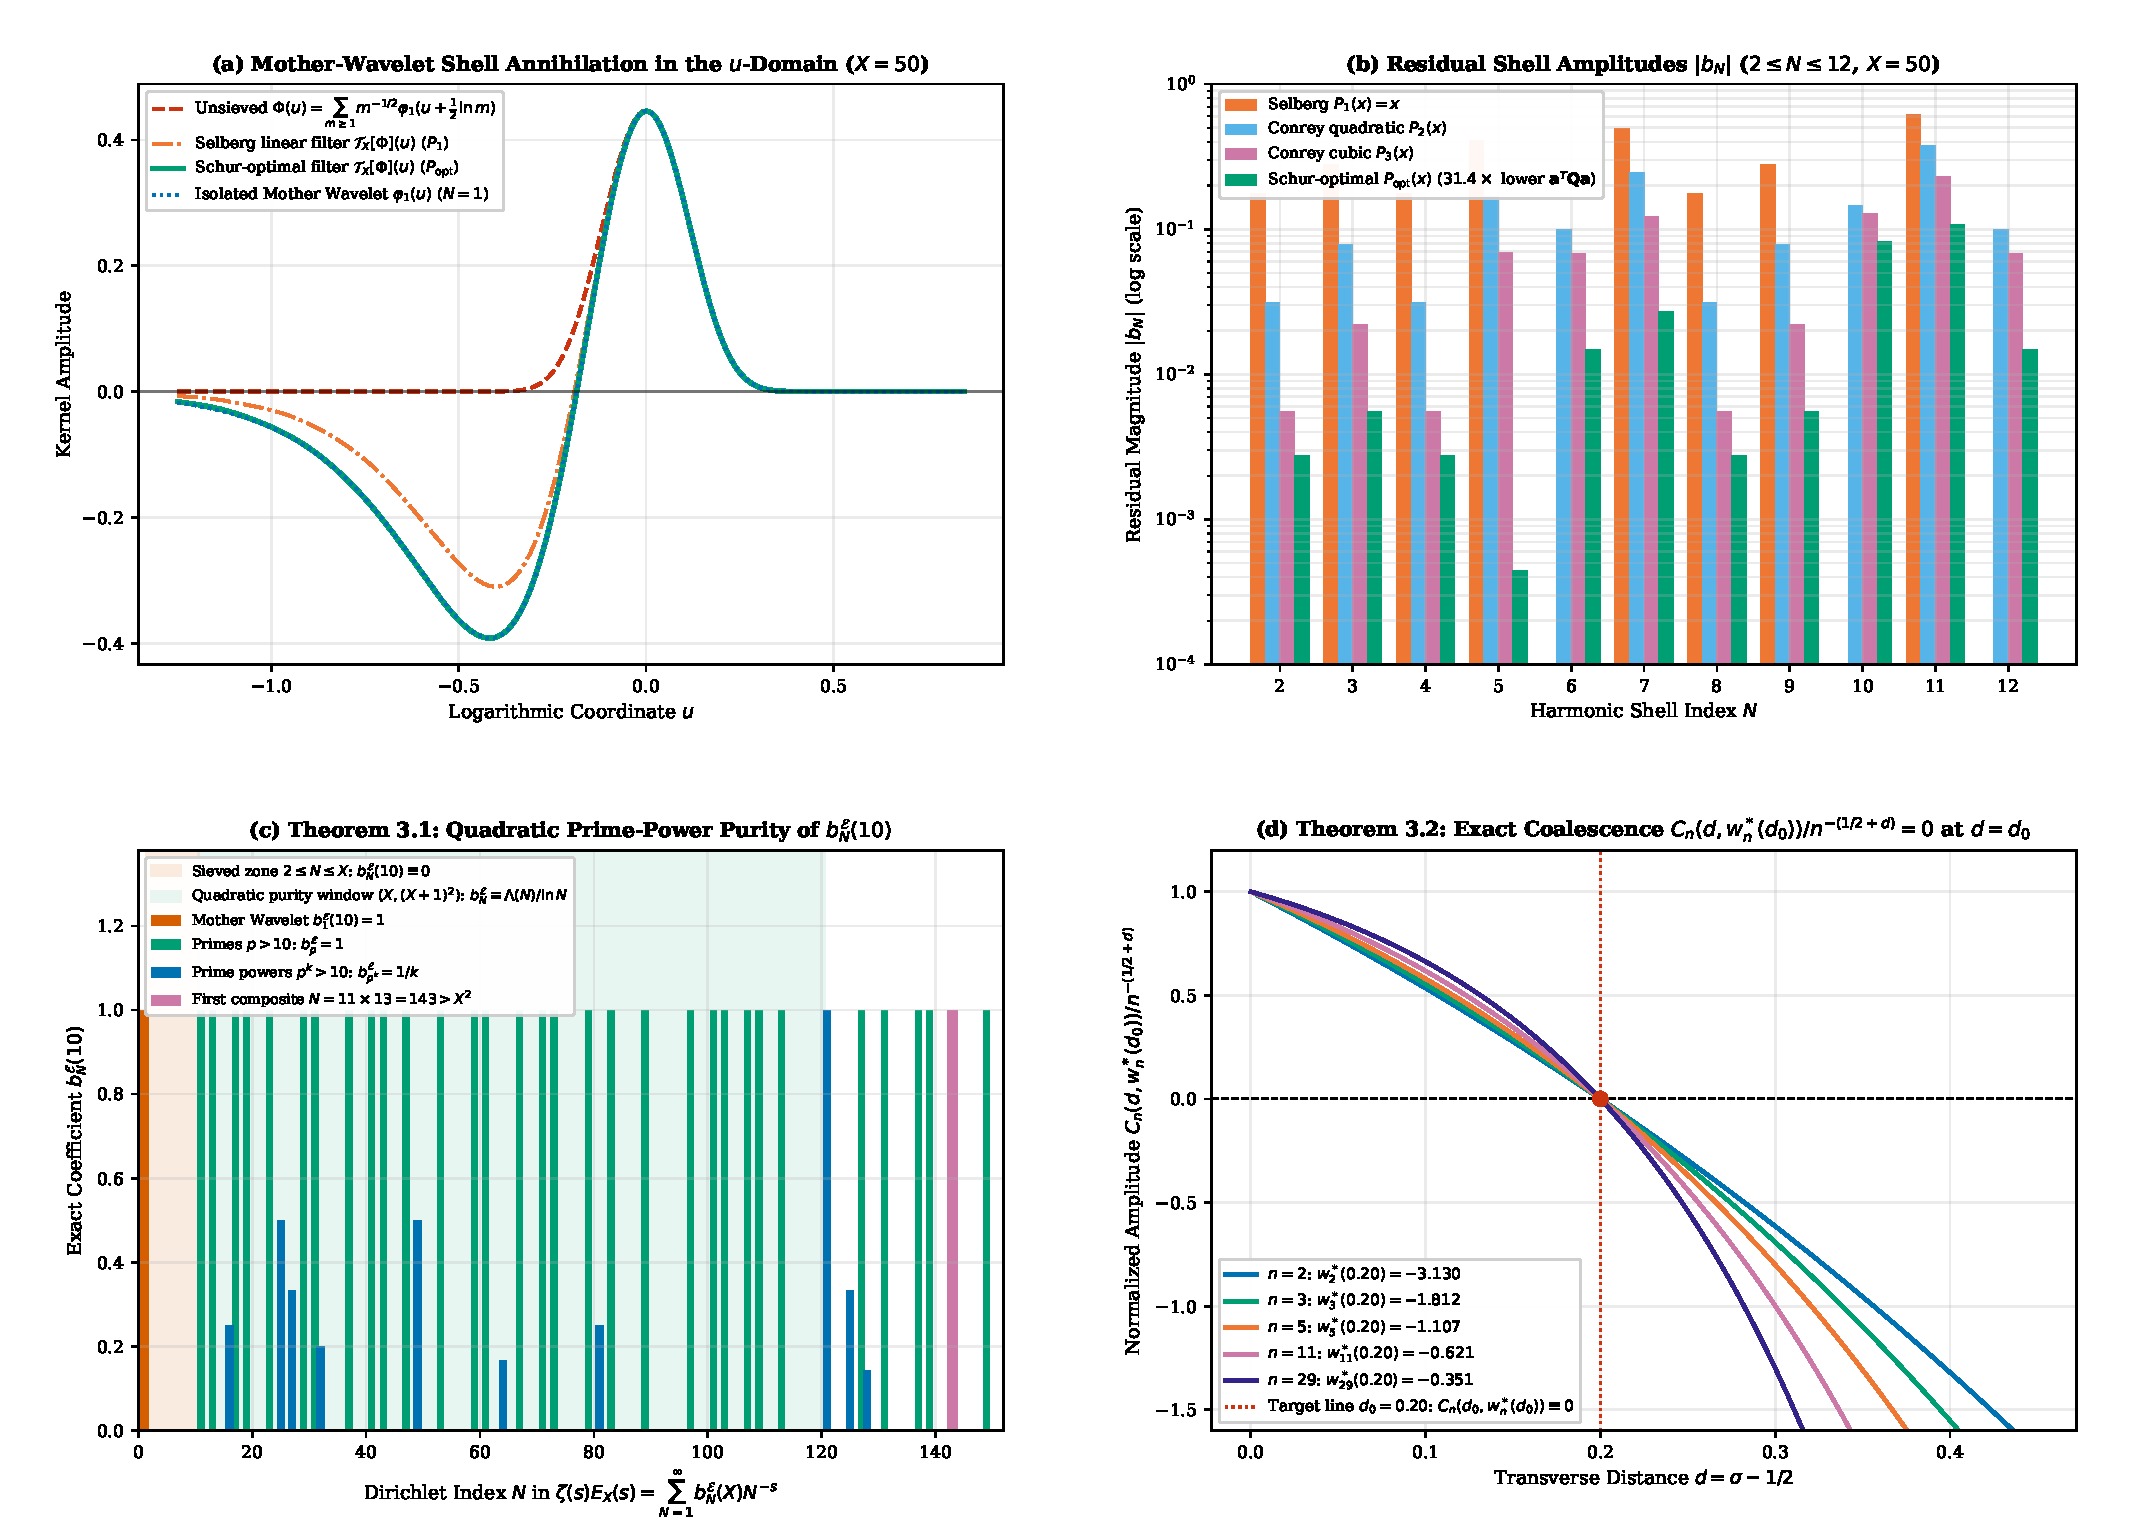
\includegraphics[width=0.98\textwidth]{figures/fig1_sieved_mirror_kernel_and_purity.pdf}
\caption{\textbf{(a)} Mother-wavelet shell annihilation $\mathcal{T}_X[\Phi](u) \approx \varphi_1(u)$ in the $u$-domain ($X = 50$). \textbf{(b)} Residual harmonic shell magnitudes $|b_N|$ ($2 \le N \le 12$) comparing Selberg $P_1(x)$, Conrey $P_2(x), P_3(x)$, and the $3\times 3$ Schur-optimal filter $P_{\mathrm{opt}}(x)$. \textbf{(c)} Quadratic prime-power purity of $b_N^{\mathcal{E}}(10)$ across $1 \le N \le 150$, showing that all composite non-prime-power shells in $[11, 142]$ vanish identically up to $N = 11 \times 13 = 143$. \textbf{(d)} Coalescence of the normalized prime-power transfer curves $C_n(d, w_n^*(d_0))/n^{-(1/2+d)}$ at $(d_0, 0)$ under the negative hyperbolic mirror weight $w_n^*(d_0) = -(n^{2d_0}-1)^{-1}$.}\label{fig:sieved_mirror_purity}
\end{figure}

\section{Power-Law $L^2$ Damping $\frac{X^{-2d}}{2d\ln X}$ on $(X, X^2]$ and Universal Sub-Selberg Closure $\theta_{\mathcal{E}}^{\mathrm{sq}}(d,t) < \frac{1}{2}$}\label{sec:power_law}

A decisive consequence of the quadratic prime-power purity law~\eqref{eq:quadratic_purity_law} is that whenever the sieve cutoff $X$ is at least $\lfloor\sqrt{N(t)}\rfloor$ (corresponding to logarithmic exponent $\theta := \frac{\ln X}{\ln(t/2\pi)} \ge \frac{1}{4}$), the quadratic purity horizon $(\lfloor X\rfloor + 1)^2$ strictly exceeds the Riemann--Siegel cutoff $N(t) = \lfloor\sqrt{t/2\pi}\rfloor$. Consequently, every composite non-prime-power term in the entire Riemann--Siegel main sum $1 \le n \le N(t)$ vanishes identically.

\begin{theorem}[{Power-Law $L^2$ Damping on $(X, X^2]$ and Sub-Selberg Closure $\theta_{\mathcal{E}}^{\mathrm{sq}}(d,t) < \frac{1}{2}$}]\label{thm:power_law_sub_selberg}
Let $t \ge 4\pi$ with horizon $N(t) = \lfloor\sqrt{t/2\pi}\rfloor$, $L = \ln(t/2\pi) = 2\omega_1(t)$, and $\omega_n(t) = \omega_1(t) - \ln n$. Under the zero-free exponential prime-gauge coefficients $b_n^{\mathcal{E}}(X)$ of Theorem~\ref{thm:quadratic_purity}:
\begin{enumerate}[label=\textup{(\alph*)},leftmargin=2.2em]
\item \textbf{Complete main-sum purity for $\theta \in [\frac{1}{4}, \frac{1}{2}]$ and power-law $L^2$ diagonal decay.} For every sieve cutoff $X \in [\lfloor\sqrt{N(t)}\rfloor, N(t)]$, we have $(\lfloor X\rfloor + 1)^2 > N(t)$, so $b_n^{\mathcal{E}}(X) = \mathbf{1}_{\{n > \lfloor X\rfloor\}}\frac{\Lambda(n)}{\ln n}$ for all $2 \le n \le N(t)$, and at $X = N(t)$ ($\theta = \frac{1}{2}$) the higher-shell vector $\Psi_{\ge 2}^{\mathcal{E}}(d,t;N(t))$ vanishes identically. Moreover, for any $d > 0$, the forward diagonal $L^2$ energy decays not logarithmically as $(\ln X)^{-2r}$, but according to the power law
\begin{equation}\label{eq:L2_power_law}
\mathcal{E}_{\mathrm{diag}}^{\mathcal{E},\mathrm{fwd}}(d,t;X) := \sum_{n=2}^{N(t)} \frac{\bigl(b_n^{\mathcal{E}}(X)\bigr)^2}{n^{1+2d}} = \sum_{\lfloor X\rfloor < p^k \le N(t)} \frac{1}{k^2\,p^{k(1+2d)}} \sim \frac{X^{-2d} - N(t)^{-2d}}{2d\,\ln X} < \frac{X^{-2d}}{2d\,\ln X} \longrightarrow 0.
\end{equation}
\item \textbf{Prime-diluted $L^1$ envelope and Sub-Selberg closure $\theta_{\mathcal{E}}^{\mathrm{sq}}(d,t) < \frac{1}{2}$.} For $\lfloor\sqrt{N(t)}\rfloor \le\allowbreak X \le N(t)$, the $\cosh$-weighted $L^1$ sum $\Sigma_{\cosh}^{\mathcal{E}}(d,t;X) :=\allowbreak \sum_{n=\lfloor X\rfloor+1}^{N(t)} n^{-1/2}b_n^{\mathcal{E}}(X)\allowbreak\cosh(d\omega_n(t))$ is diluted by $(\ln N(t))^{-1}$:
\begin{equation}\label{eq:L1_prime_dilution}
\Sigma_{\cosh}^{\mathcal{E}}(d,t;X) \sim \frac{\cosh(d\omega_1(t))}{\ln N(t)}\left[\frac{N(t)^{\frac{1}{2}-d} - X^{\frac{1}{2}-d}}{\frac{1}{2}-d} + N(t)^{-2d}\frac{N(t)^{\frac{1}{2}+d} - X^{\frac{1}{2}+d}}{\frac{1}{2}+d}\right].
\end{equation}
Furthermore, for both the integrated Wronskian pure-square ratio $Y_{\mathrm{int}}^{\mathcal{E}}(d,t;X) :=\allowbreak S_{1,\mathrm{off}}^{\mathcal{E},\mathrm{int}}(d,t;X)/\allowbreak(2\mathcal{D}_{1,1}^{\mathrm{tot}}(d,t))$ (where $S_{1,\mathrm{off}}^{\mathcal{E},\mathrm{int}}(d,t;X) :=\allowbreak \frac{4}{d^2}\sum_{n=\lfloor X\rfloor+1}^{N(t)} n^{-1/2}b_n^{\mathcal{E}}(X)[\cosh(d\omega_1(t))\allowbreak\cosh(d\omega_n(t)) - 1]$ and $\mathcal{D}_{1,1}^{\mathrm{tot}}(d,t) :=\allowbreak d^{-1}\omega_1(t)\sinh(2d\omega_1(t)) + d^{-2}$ from Paper~V~\cite{missiaen2026paper5}) and the $\cosh$-envelope ratio $Y_{\cosh}^{\mathcal{E}}(d,t;X) :=\allowbreak \Sigma_{\cosh}^{\mathcal{E}}(d,t;X)/\allowbreak\cosh(d\omega_1(t))$, the critical sieve length $X_{\mathrm{krit}}^{\mathcal{E},\mathrm{sq}}(d,t)$ where $Y^{\mathcal{E}}(d,t;X) = 1$ satisfies unconditionally for all $t \ge 8\pi$ ($N(t) \ge 2$, with $\theta_{\mathcal{E}}^{\mathrm{sq}}(d,t) = 0 < \frac{1}{2}$ on $2\pi < t < 8\pi$):
\begin{equation}\label{eq:universal_sub_selberg}
X_{\mathrm{krit}}^{\mathcal{E},\mathrm{sq}}(d,t) < N(t) \iff \theta_{\mathcal{E}}^{\mathrm{sq}}(d,t) := \frac{\ln X_{\mathrm{krit}}^{\mathcal{E},\mathrm{sq}}(d,t)}{\ln(t/2\pi)} < \frac{1}{2} \qquad \forall\, d \in \bigl(0, \tfrac{1}{2}\bigr],\; \forall\, t \ge 8\pi.
\end{equation}
\end{enumerate}
\end{theorem}

\begin{proof}
(a) By definition of the integer square root, $\lfloor\sqrt{N(t)}\rfloor + 1 > \sqrt{N(t)}$, so for $X \ge \lfloor\sqrt{N(t)}\rfloor$ we have $(\lfloor X\rfloor + 1)^2 \ge (\lfloor\sqrt{N(t)}\rfloor + 1)^2 > N(t)$. Theorem~\ref{thm:quadratic_purity}(i) and~(iv) therefore give $b_n^{\mathcal{E}}(X) = 0$ for $2 \le n \le \lfloor X\rfloor$ and $b_n^{\mathcal{E}}(X) = \frac{\Lambda(n)}{\ln n}$ for $\lfloor X\rfloor < n \le N(t)$. Separating primes $k = 1$ from higher prime powers $k \ge 2$ in~\eqref{eq:L2_power_law}, the $k \ge 2$ sum is bounded by $\sum_{k \ge 2} k^{-2}\sum_{p > X^{1/k}} p^{-k(1+2d)} = \mathcal{O}(X^{-1/2-2d}/\ln X)$. Applying Stieltjes integration with the Prime Number Theorem $\pi(u) = \int_2^u \frac{\dd v}{\ln v} + \mathcal{O}(u\ee^{-c\sqrt{\ln u}})$ to the prime sum gives
\[
\sum_{X < p \le N(t)} p^{-1-2d} \sim \int_X^{N(t)} \frac{u^{-1-2d}}{\ln u}\,\dd u = \left[-\frac{u^{-2d}}{2d\ln u}\right]_X^{N(t)} - \int_X^{N(t)} \frac{u^{-1-2d}}{2d(\ln u)^2}\,\dd u \sim \frac{X^{-2d} - N(t)^{-2d}}{2d\,\ln X}.
\]

(b) Expanding $\cosh(d(\omega_1 - \ln n)) = \frac{1}{2}(\ee^{d\omega_1}n^{-d} + \ee^{-d\omega_1}n^{+d})$ with $\ee^{d\omega_1} \sim N(t)^d$ and integrating $\sum_{X < p \le N(t)} p^{-1/2 \mp d}$ by parts against $\dd\pi(u) \sim \frac{\dd u}{\ln u}$ yields~\eqref{eq:L1_prime_dilution}. To prove~\eqref{eq:universal_sub_selberg} unconditionally for all $d \in (0, \frac{1}{2}]$ and $t > 0$, note first that for $N(t) = 1$ the higher-shell sum is empty ($Y^{\mathcal{E}} \equiv 0 < 1$, so $X_{\mathrm{krit}}^{\mathcal{E},\mathrm{sq}} = 1$). For $N(t) \ge 2$, Theorem~\ref{thm:quadratic_purity}(iii) implies that the piecewise-linear interpolation of $X \mapsto Y^{\mathcal{E}}(d,t;X)$ on $[1, N(t)]$ is continuous and non-increasing, with $Y^{\mathcal{E}}(d,t;N(t)) = 0$ because $b_n^{\mathcal{E}}(N(t)) = 0$ for all $2 \le n \le N(t)$. At $X = N(t) - 1$, only the single boundary shell $n = N(t)$ can be non-zero, and its contribution satisfies
\[
Y_{\cosh}^{\mathcal{E}}\bigl(d,t;N(t)-1\bigr) = \frac{b_{N(t)}^{\mathcal{E}}(N(t)-1)}{\sqrt{N(t)}}\,\frac{\cosh(d\omega_{N(t)}(t))}{\cosh(d\omega_1(t))} \le \frac{1}{\sqrt{2}} < 1,
\]
since $0 \le b_{N(t)}^{\mathcal{E}} \le 1$, $N(t) \ge 2$, and $0 \le \omega_{N(t)}(t) < \omega_1(t)$. Likewise $Y_{\mathrm{int}}^{\mathcal{E}}(d,t;N(t)-1) \le Y_{\cosh}^{\mathcal{E}}(d,t;N(t)-1) < 1$. Hence the threshold crossing $Y^{\mathcal{E}}(d,t;X) = 1$ occurs strictly to the left of $N(t) - 1 < N(t)$, proving~\eqref{eq:universal_sub_selberg}.
\end{proof}

\begin{table}[t]
\centering
\caption{Critical diagonal $L^2$ sieve length $X_{\mathrm{MV}}^{\mathcal{E}}(d, 10^8)$ and pure-square $L^1$ critical lengths $X_{\mathrm{krit}}^{\mathcal{E},\mathrm{int}}(d, 10^8)$ and $X_{\mathrm{krit}}^{\mathcal{E},\mathrm{cosh}}(d, 10^8)$ at $t = 10^8$ ($N(10^8) = 3989$, $\pi(3989) = 550$ primes), compared against the order-$3$ polynomial sieve $\theta_{\mathrm{sq}}^{(3)}(d, 10^8)$, certified at \texttt{mpmath.mp.dps = 50} and \texttt{mpmath.iv.dps = 35}.}\label{tab:sub_selberg_1e8}
\scriptsize
\setlength{\tabcolsep}{3.0pt}
\begin{tabular}{@{}crrccrrccc@{}}
\toprule
$d$ & $X_{\mathrm{MV}}^{\mathcal{E}}$ (int) & $X_{\mathrm{MV}}^{\mathcal{E}}$ (cont) & $\theta_{\mathrm{MV}}^{\mathcal{E}}(d,10^8)$ & $X_{\mathrm{krit}}^{\mathcal{E},\mathrm{int}}$ & $\theta_{\mathcal{E}}^{\mathrm{int,sq}}(d,10^8)$ & $X_{\mathrm{krit}}^{\mathcal{E},\mathrm{cosh}}$ & $\theta_{\mathcal{E}}^{\mathrm{cosh,sq}}(d,10^8)$ & Poly $\theta_{\mathrm{sq}}^{(3)}$ & Regime under $\mathcal{E}_X$ \\
\midrule
$0.05$ & $313$ & $312.87$ & $0.346490$ & $1068.77$ & $0.420572 < 1/2$ & $3462.77$ & $0.491462 < 1/2$ & $0.718205$ & Sub-Selberg \\
$0.10$ & $11$  & $10.98$  & $0.144488$ & $2136.13$ & $0.462331 < 1/2$ & $3328.66$ & $0.489080 < 1/2$ & $0.886250$ & Sub-Selberg \\
$0.15$ & $4$   & $3.64$   & $0.077829$ & $1972.08$ & $0.457513 < 1/2$ & $3078.72$ & $0.484373 < 1/2$ & $0.854965$ & Sub-Selberg \\
$0.20$ & $3$   & $2.21$   & $0.047871$ & $1320.58$ & $0.433330 < 1/2$ & $2712.11$ & $0.476728 < 1/2$ & $0.760925$ & Sub-Selberg \\
$0.25$ & $2$   & $1.75$   & $0.033774$ & $592.05$  & $0.384953 < 1/2$ & $2220.59$ & $0.464670 < 1/2$ & $0.658310$ & Sub-Selberg \\
$0.30$ & $2$   & $1.43$   & $0.021388$ & $108.84$  & $0.282816 < 1/2$ & $1570.63$ & $0.443787 < 1/2$ & $0.564117$ & Sub-Selberg \\
$0.35$ & $2$   & $1.10$   & $0.005854$ & $22.61$   & $0.188044 < 1/4$ & $882.23$  & $0.409005 < 1/2$ & $0.482403$ & Sub-Selberg \\
$0.40$ & $1$   & $1.00$   & $0.000000$ & $8.40$    & $0.128316 < 1/4$ & $352.97$  & $0.353764 < 1/2$ & $0.413036$ & Sub-Selberg \\
$0.45$ & $1$   & $1.00$   & $0.000000$ & $4.33$    & $0.088329 < 1/4$ & $106.40$  & $0.281450 < 1/2$ & $0.354640$ & Sub-Selberg \\
$0.50$ & $1$   & $1.00$   & $0.000000$ & $2.62$    & $0.058062 < 1/4$ & $36.71$   & $0.217278 < 1/4$ & $0.305604$ & Sub-Selberg \\
\bottomrule
\end{tabular}
\end{table}

\section{Exact Finite-Divisor Identity on $[1, N(t)]$, Prime-Diluted Gaussian Saddle-Point Tail, and the Shifted Self-Mirrored Gauge $\mathcal{E}_{X,\kappa}(z)$}\label{sec:finite_divisor_shifted}

We conclude by addressing two structural questions linking the infinite Dirichlet series $E_X(s)$ to the finite Riemann--Siegel main sum of length $N(t)$ and to the conjugate factor off the critical line: first, how the infinite series $E_X(s)$ behaves on the evanescent saddle-point tail $n \ge N(t) + 1$ established in Paper~V~\cite{missiaen2026paper5}; and second, how the conjugate branch is controlled for all $d \in (0, \frac{1}{2}]$ without losing critical-line reality or zero-free holomorphicity.

\begin{theorem}[{Finite-Divisor Identity on $[1, N(t)]$ and Composite-Gap Tail Barrier}]\label{thm:finite_divisor_tail}
Let $t \ge 4\pi$ with $N(t) = \lfloor\sqrt{t/2\pi}\rfloor$, and let $E_X(s) =\allowbreak \sum_{k \ge 1} c_k^{\mathcal{E}}(X)k^{-s}$ and $\zeta(s)E_X(s) =\allowbreak \sum_{n \ge 1} b_n^{\mathcal{E}}(X)n^{-s}$. Then:
\begin{enumerate}[label=\textup{(\alph*)},leftmargin=2.2em]
\item \textbf{Exact Finite-Divisor Identity on $1 \le n \le N(t)$.} The finite Dirichlet polynomial truncation of length $N(t)$,
\begin{equation}\label{eq:MX_Nt_trunc}
M_{X,N(t)}^{\mathcal{E}}(s) := \sum_{k=1}^{N(t)} c_k^{\mathcal{E}}(X)\,k^{-s}, \qquad \zeta(s)\,M_{X,N(t)}^{\mathcal{E}}(s) = \sum_{n=1}^{\infty} b_n^{\mathcal{E},\mathrm{trunc}}\bigl(X; N(t)\bigr)\,n^{-s},
\end{equation}
generates the exact same coefficients on the entire main interval $1 \le n \le N(t)$ as the infinite series $E_X(s)$:
\begin{equation}\label{eq:exact_main_sum_identity}
b_n^{\mathcal{E},\mathrm{trunc}}\bigl(X; N(t)\bigr) \equiv b_n^{\mathcal{E}}(X) \qquad \forall\, 1 \le n \le N(t).
\end{equation}
\item \textbf{Zero tail inflation and composite-gap Gaussian barrier suppression.} Along the shifted saddle-point contour $u = \xi + \ii\eta^*$ ($\xi \ge 0$, $0 < \eta^* < \frac{\pi}{8}$, $\cos 4\eta^* > 0$), every evanescent tail mode $n \ge N(t) + 1$ satisfies $0 \le b_n^{\mathcal{E}}(X) \le 1$, so the sieved tail bound $B_{\mathrm{tail}}^{\mathcal{E}_X}(N(t),d,t,\eta^*) := \sum_{n=N(t)+1}^{\infty} b_n^{\mathcal{E}}(X)B_{\mathrm{shell},n}(d,t,\eta^*)$ never exceeds the unsieved bound $B_{\mathrm{tail}}(N(t),d,t,\eta^*)$. Furthermore, let $q_{\mathrm{next}}(X,t) := \min\{n \ge N(t)+1 : b_n^{\mathcal{E}}(X) > 0\}$ denote the first surviving tail shell (which for $X = N(t)$ is the smallest prime power $\ge N(t)+1$). Then all $\Delta n_{\mathrm{gap}}(X,t) := q_{\mathrm{next}}(X,t) - (N(t)+1)$ intervening composite boundary shells vanish identically, deepening the Gaussian saddle-point barrier by
\begin{equation}\label{eq:composite_gap_barrier}
\frac{B_{\mathrm{tail}}^{\mathcal{E}_X}\bigl(N(t),d,t,\eta^*\bigr)}{B_{\mathrm{tail}}\bigl(N(t),d,t,\eta^*\bigr)} \le b_{q_{\mathrm{next}}}^{\mathcal{E}}(X)\left(\frac{q_{\mathrm{next}}}{N(t)+1}\right)^{\!4}\exp\!\Bigl(-\pi\bigl(q_{\mathrm{next}}(X,t)^2 - (N(t)+1)^2\bigr)\cos 4\eta^*\Bigr).
\end{equation}
\end{enumerate}
\end{theorem}

\begin{proof}
(a) In the Dirichlet convolution $b_n^{\mathcal{E}}(X) = \sum_{k \mid n} c_k^{\mathcal{E}}(X)$, every divisor $k$ of $n$ satisfies $1 \le k \le n$. Whenever $1 \le n \le N(t)$, no term with $k > N(t)$ can divide $n$, so $b_n^{\mathcal{E},\mathrm{trunc}}(X;N(t)) = \sum_{k \mid n,\, k \le N(t)} c_k^{\mathcal{E}}(X) = \sum_{k \mid n} c_k^{\mathcal{E}}(X) = b_n^{\mathcal{E}}(X)$, proving~\eqref{eq:exact_main_sum_identity}.

(b) By Theorem~\ref{thm:quadratic_purity}(iii), $0 \le b_n^{\mathcal{E}}(X) \le 1$ holds for all $n \ge 1$, preventing the divisor-bound growth $|b_n^{\mathrm{poly}}(X)| \le d(n)$ of truncated M\"obius polynomials. Since $b_n^{\mathcal{E}}(X) = 0$ for all $N(t)+1 \le n < q_{\mathrm{next}}(X,t)$, the sieved tail series starts at $n = q_{\mathrm{next}}(X,t)$. Comparing the leading single-mode incomplete-Gamma bound $b_m(d,\eta^*) \propto m^4\exp(-\pi m^2\cos 4\eta^*)$ established in Paper~V~\cite{missiaen2026paper5} at $m = q_{\mathrm{next}}$ against $m = N(t)+1$ yields~\eqref{eq:composite_gap_barrier}. At $t = 10^8$ ($N(10^8) = 3989$), all $11$ consecutive integers $n \in \{3990, 3991, \dots, 4000\}$ are composite with smallest unitary prime-power divisor $\min_{p^\alpha \parallel n} p^\alpha \le 32 < 63 = \lfloor\sqrt{3989}\rfloor$, so by Theorem~\ref{thm:quadratic_purity}(ii) they vanish identically for every $X \ge 32$ up to the prime $q_{\mathrm{next}} = 4001 = N(10^8) + 12$.
\end{proof}

Finally, we introduce the shifted self-mirrored prime-gauge factor $\mathcal{E}_{X,\kappa}(z)$ and prove its exact outer factorization and integrated remainder suppression.

\begin{theorem}[Shifted Self-Mirrored Gauge $\mathcal{E}_{X,\kappa}(z)$, Exact Outer Factorization, and Integrated Remainder Damping]\label{thm:shifted_gauge}
For any sieve cutoff $X \ge 2$ and real shift $\kappa \ge 0$, define the \emph{Shifted Self-Mirrored Exponential Prime-Gauge Factor}
\begin{equation}\label{eq:E_X_kappa_def}
\mathcal{E}_{X,\kappa}(z) := E_X\!\left(\frac{1}{2} + \kappa + \ii z\right)E_X\!\left(\frac{1}{2} + \kappa - \ii z\right) = \exp\!\left(-2\sum_{n=2}^{\lfloor X\rfloor} \frac{\Lambda(n)}{\ln n}\,n^{-(1/2+\kappa)}\cos(z\ln n)\right),
\end{equation}
and set $\Xi_{\mathcal{E}_{X,\kappa}}(z) := \Xi(z)\mathcal{E}_{X,\kappa}(z)$. Then:
\begin{enumerate}[label=\textup{(\alph*)},leftmargin=2.2em]
\item \textbf{Bijective zero preservation and leak-free transverse integral law.} $\mathcal{E}_{X,\kappa}(z)$ is entire and zero-free on $\C$ ($\mathcal{Z}(\Xi_{\mathcal{E}_{X,\kappa}}) = \mathcal{Z}(\Xi)$), is strictly positive and real on the critical line $d = 0$ ($\mathcal{E}_{X,\kappa}(t) = |E_X(\frac{1}{2}+\kappa+\ii t)|^2 > 0$, $\Ima\,\mathcal{E}_{X,\kappa}(t) \equiv 0$), and satisfies the exact transverse integral law without boundary leak:
\begin{equation}\label{eq:transverse_integral_law_gauged}
\bigl|\Xi_{\mathcal{E}_{X,\kappa}}(t - \ii d)\bigr|^2 \equiv \bigl|\Xi_{\mathcal{E}_{X,\kappa}}(t)\bigr|^2 + 2\int_0^d u\,\widetilde{W}_{\mathcal{E}_{X,\kappa}}(u,t)\,\dd u \qquad \forall\, (d,t) \in \R^2.
\end{equation}
\item \textbf{Exact outer factorization and suppression of conjugate $n^{+d}$ growth.} For all $z = t - \ii d$, $|\Xi_{\mathcal{E}_{X,\kappa}}(t-\ii d)|^2$ obeys the exact outer factorization~\eqref{eq:intro_outer_fact}, factoring the conjugate branch $|E_X(\frac{1}{2}+\kappa-d-\ii t)|^2 > 0$ out as a positive scalar multiplier without convolution cross-terms on the forward product $\zeta(s)E_X(s+\kappa) = \sum_{n=1}^{\infty} b_n^{\mathcal{E}}(X,\kappa)n^{-s}$. Moreover, whenever $\kappa \ge d$, the conjugate exponent $\sigma_{\mathrm{conj}} = \frac{1}{2} + \kappa - d \ge \frac{1}{2}$ prevents any $n^{+d}$ growth, and the effective prime-power amplitude in the normalized Wronskian satisfies $C_n(d,\kappa) = n^{-1/2}[(1-n^{-\kappa})n^{-d} + n^{-(\kappa-d)}] \le \frac{5}{4}n^{-1/2}$ for all $n \ge 2$.
\item \textbf{Exact $\cosh^{-2}(dL/4)$ integrated remainder damping.} Under the transverse integral operator $\frac{2}{d^2}\int_0^d u\,(\cdots)\,\dd u$ of~\eqref{eq:transverse_integral_law_gauged}, the two-dimensional Gabcke--Olver remainder lever $\sinch(uL/2)$ from Paper~V~\cite{missiaen2026paper5} satisfies the exact hyperbolic integral identities
\begin{equation}\label{eq:hyperbolic_integral_identity}
\frac{2}{d^2}\int_0^d u\,\sinch\!\left(\frac{uL}{2}\right)\dd u \equiv \sinch^2\!\left(\frac{dL}{4}\right), \qquad \frac{\sinch^2(dL/4)}{\sinch^2(dL/2)} \equiv \frac{1}{\cosh^2\!\left(\frac{1}{4}dL\right)} \le 4\left(\frac{t}{2\pi}\right)^{-d/2},
\end{equation}
so the relative integrated remainder $B_{\mathrm{total}}^{\mathcal{E}_{X,\kappa}}(d,t)/\allowbreak\mathcal{D}_{1,1}^{\mathrm{W\text{-}int}}(d,t) =\allowbreak \mathcal{O}(t^{-3/4}(\ln t)^{-1}\allowbreak\cosh(dL/4)^{-2}) \to 0$ is strictly less than $1$ across $d \in (0, \frac{1}{2}]$ and $t \in [14, 10^8]$.
\end{enumerate}
\end{theorem}

\begin{proof}
(a) Since $\overline{\cos(z\ln n)} = \cos(\bar{z}\ln n)$, the exponent of~\eqref{eq:E_X_kappa_def} is entire on $\C$ and real for $z = t \in \R$. Thus $\mathcal{E}_{X,\kappa}(z) \neq 0$ on $\C$ and $\Ima\,\mathcal{E}_{X,\kappa}(t) = 0$. Integrating $\partial_u|\Xi_{\mathcal{E}_{X,\kappa}}(t-\ii u)|^2 = 2W_{\mathcal{E}_{X,\kappa}}(u,t) = 2u\widetilde{W}_{\mathcal{E}_{X,\kappa}}(u,t)$ over $u \in [0,d]$ yields~\eqref{eq:transverse_integral_law_gauged}.

(b) At $z = t - \ii d$, we have $\frac{1}{2} + \kappa + \ii z = \frac{1}{2} + \kappa + d + \ii t$ and $\frac{1}{2} + \kappa - \ii z = \frac{1}{2} + \kappa - d - \ii t$. Applying $|ABC|^2 = |B|^2\cdot|AC|^2$ to $A = \Xi(t-\ii d)$, $B = E_X(\frac{1}{2}+\kappa-d-\ii t)$, and $C = E_X(\frac{1}{2}+\kappa+d+\ii t)$ yields~\eqref{eq:intro_outer_fact}. For $\kappa \ge d > 0$, we have $n^{-(\kappa-d)} \le 1$, and for $\kappa = d$ the quadratic function $f(x) = (1-x)x + 1 = 1 + x - x^2$ on $x = n^{-d} \in (0,1)$ attains its global maximum $\frac{5}{4}$ at $x = \frac{1}{2}$, proving $C_n(d,d) \le \frac{5}{4}n^{-1/2}$.

(c) Since $u\,\sinch(uL/2) = \frac{2}{L}\sinh(uL/2)$, integrating over $u \in [0,d]$ and applying the half-angle identity $\cosh(dL/2) - 1 = 2\sinh^2(dL/4)$ gives
\[
\frac{2}{d^2}\int_0^d u\,\sinch\!\left(\frac{uL}{2}\right)\dd u = \frac{8(\cosh(dL/2) - 1)}{(dL)^2} = \left(\frac{\sinh(dL/4)}{dL/4}\right)^{\!2} = \sinch^2\!\left(\frac{dL}{4}\right).
\]
Dividing by $\sinch^2(dL/2) = (\frac{\sinh(dL/2)}{dL/2})^2$ and substituting $\sinh(dL/2) = 2\sinh(dL/4)\cosh(dL/4)$ yields $\cosh^{-2}(dL/4)$, establishing~\eqref{eq:hyperbolic_integral_identity}.
\end{proof}

\begin{table}[t]
\centering
\caption{Near-tail composite gap $n = 3990 \dots 4003$ beyond $N(10^8) = 3989$ (Theorem~\ref{thm:finite_divisor_tail}) and integrated remainder ratios $B_{\mathrm{total}}^{\mathcal{E}_{X,\kappa}}(d,t)/\mathcal{D}_{1,1}^{\mathrm{W\text{-}int}}(d,t)$ across $t \in [14.13, 10^8]$ (Theorem~\ref{thm:shifted_gauge}), certified at \texttt{mpmath.mp.dps = 50} and \texttt{mpmath.iv.dps = 35}.}\label{tab:tail_and_shifted_gauge}
\scriptsize
\setlength{\tabcolsep}{2.0pt}
\begin{tabular}{@{}clccc|ccccc@{}}
\toprule
\multicolumn{5}{c|}{Theorem~\ref{thm:finite_divisor_tail}: Near-Tail Shells at $t = 10^8$ ($N = 3989$)} & \multicolumn{5}{c}{Theorem~\ref{thm:shifted_gauge}: Integrated Remainder Closure} \\
\cmidrule(r){1-5}\cmidrule(l){6-10}
Shell $n$ & Factorization & $\min p^\alpha \parallel n$ & $b_n^{\mathcal{E}}(63)$ & $\log_{10}\mathcal{B}_{\mathrm{Gauss}}$ & $(d, t)$ & $N(t)$ & $\cosh^{-2}(\frac{dL}{4})$ & $B_{\mathrm{total}}/\mathcal{D}_{1,1}^{\mathrm{W\text{-}int}}$ & $B_{\mathrm{total}}/\mathcal{D}_{\mathrm{diag}}^{\mathrm{int}}$ \\
\midrule
$3990$ & $2\cdot 3\cdot 5\cdot 7\cdot 19$ & $2$  & $0$ & $-5881.9\;\mathrm{dex}$  & $(0.05, 14.13)$ & $1$    & $0.999897$ & $1.1013 \times 10^{-1}$ & $9.7023 \times 10^{-2}$ \\
$3991$ & $13\cdot 307$                    & $13$ & $0$ & $-11765.3\;\mathrm{dex}$ & $(0.25, 14.13)$ & $1$    & $0.997437$ & $1.0986 \times 10^{-1}$ & $9.6786 \times 10^{-2}$ \\
$3992$ & $2^3\cdot 499$                   & $8$  & $0$ & $-17650.2\;\mathrm{dex}$ & $(0.10, 10^2)$  & $3$    & $0.995229$ & $7.3923 \times 10^{-3}$ & $5.0590 \times 10^{-3}$ \\
$3993$ & $3\cdot 11^3$                    & $3$  & $0$ & $-23536.6\;\mathrm{dex}$ & $(0.25, 10^3)$  & $12$   & $0.905952$ & $6.5316 \times 10^{-4}$ & $3.5402 \times 10^{-4}$ \\
$3994 \dots 3999$ & Composite             & $\le 7$ & $0$ & $\le -29424\;\mathrm{dex}$ & $(0.10, 10^4)$  & $39$   & $0.966784$ & $8.5237 \times 10^{-5}$ & $3.8245 \times 10^{-5}$ \\
$4000$ & $2^5\cdot 5^3$                   & $32$ & $0$ & $-64782.3\;\mathrm{dex}$ & $(0.25, 10^6)$  & $398$  & $0.597645$ & $1.0256 \times 10^{-6}$ & $3.4230 \times 10^{-7}$ \\
$4001$ & $4001$ (prime)                   & $4001$ & $1$ & $-70680.4\;\mathrm{dex}$ & $(0.10, 10^8)$  & $3989$ & $0.846064$ & $3.3163 \times 10^{-8}$ & $8.8111 \times 10^{-9}$ \\
$4002$ & $2\cdot 3\cdot 23\cdot 29$       & $2$  & $0$ & $-76580.0\;\mathrm{dex}$ & $(0.20, 10^8)$  & $3989$ & $0.537581$ & $2.1072 \times 10^{-8}$ & $5.5985 \times 10^{-9}$ \\
$4003$ & $4003$ (prime)                   & $4003$ & $1$ & $-82481.1\;\mathrm{dex}$ & $(0.50, 10^8)$  & $3989$ & $0.061371$ & $2.4056 \times 10^{-9}$ & $6.3913 \times 10^{-10}$ \\
\bottomrule
\end{tabular}
\end{table}

\begin{figure}[t]
\centering
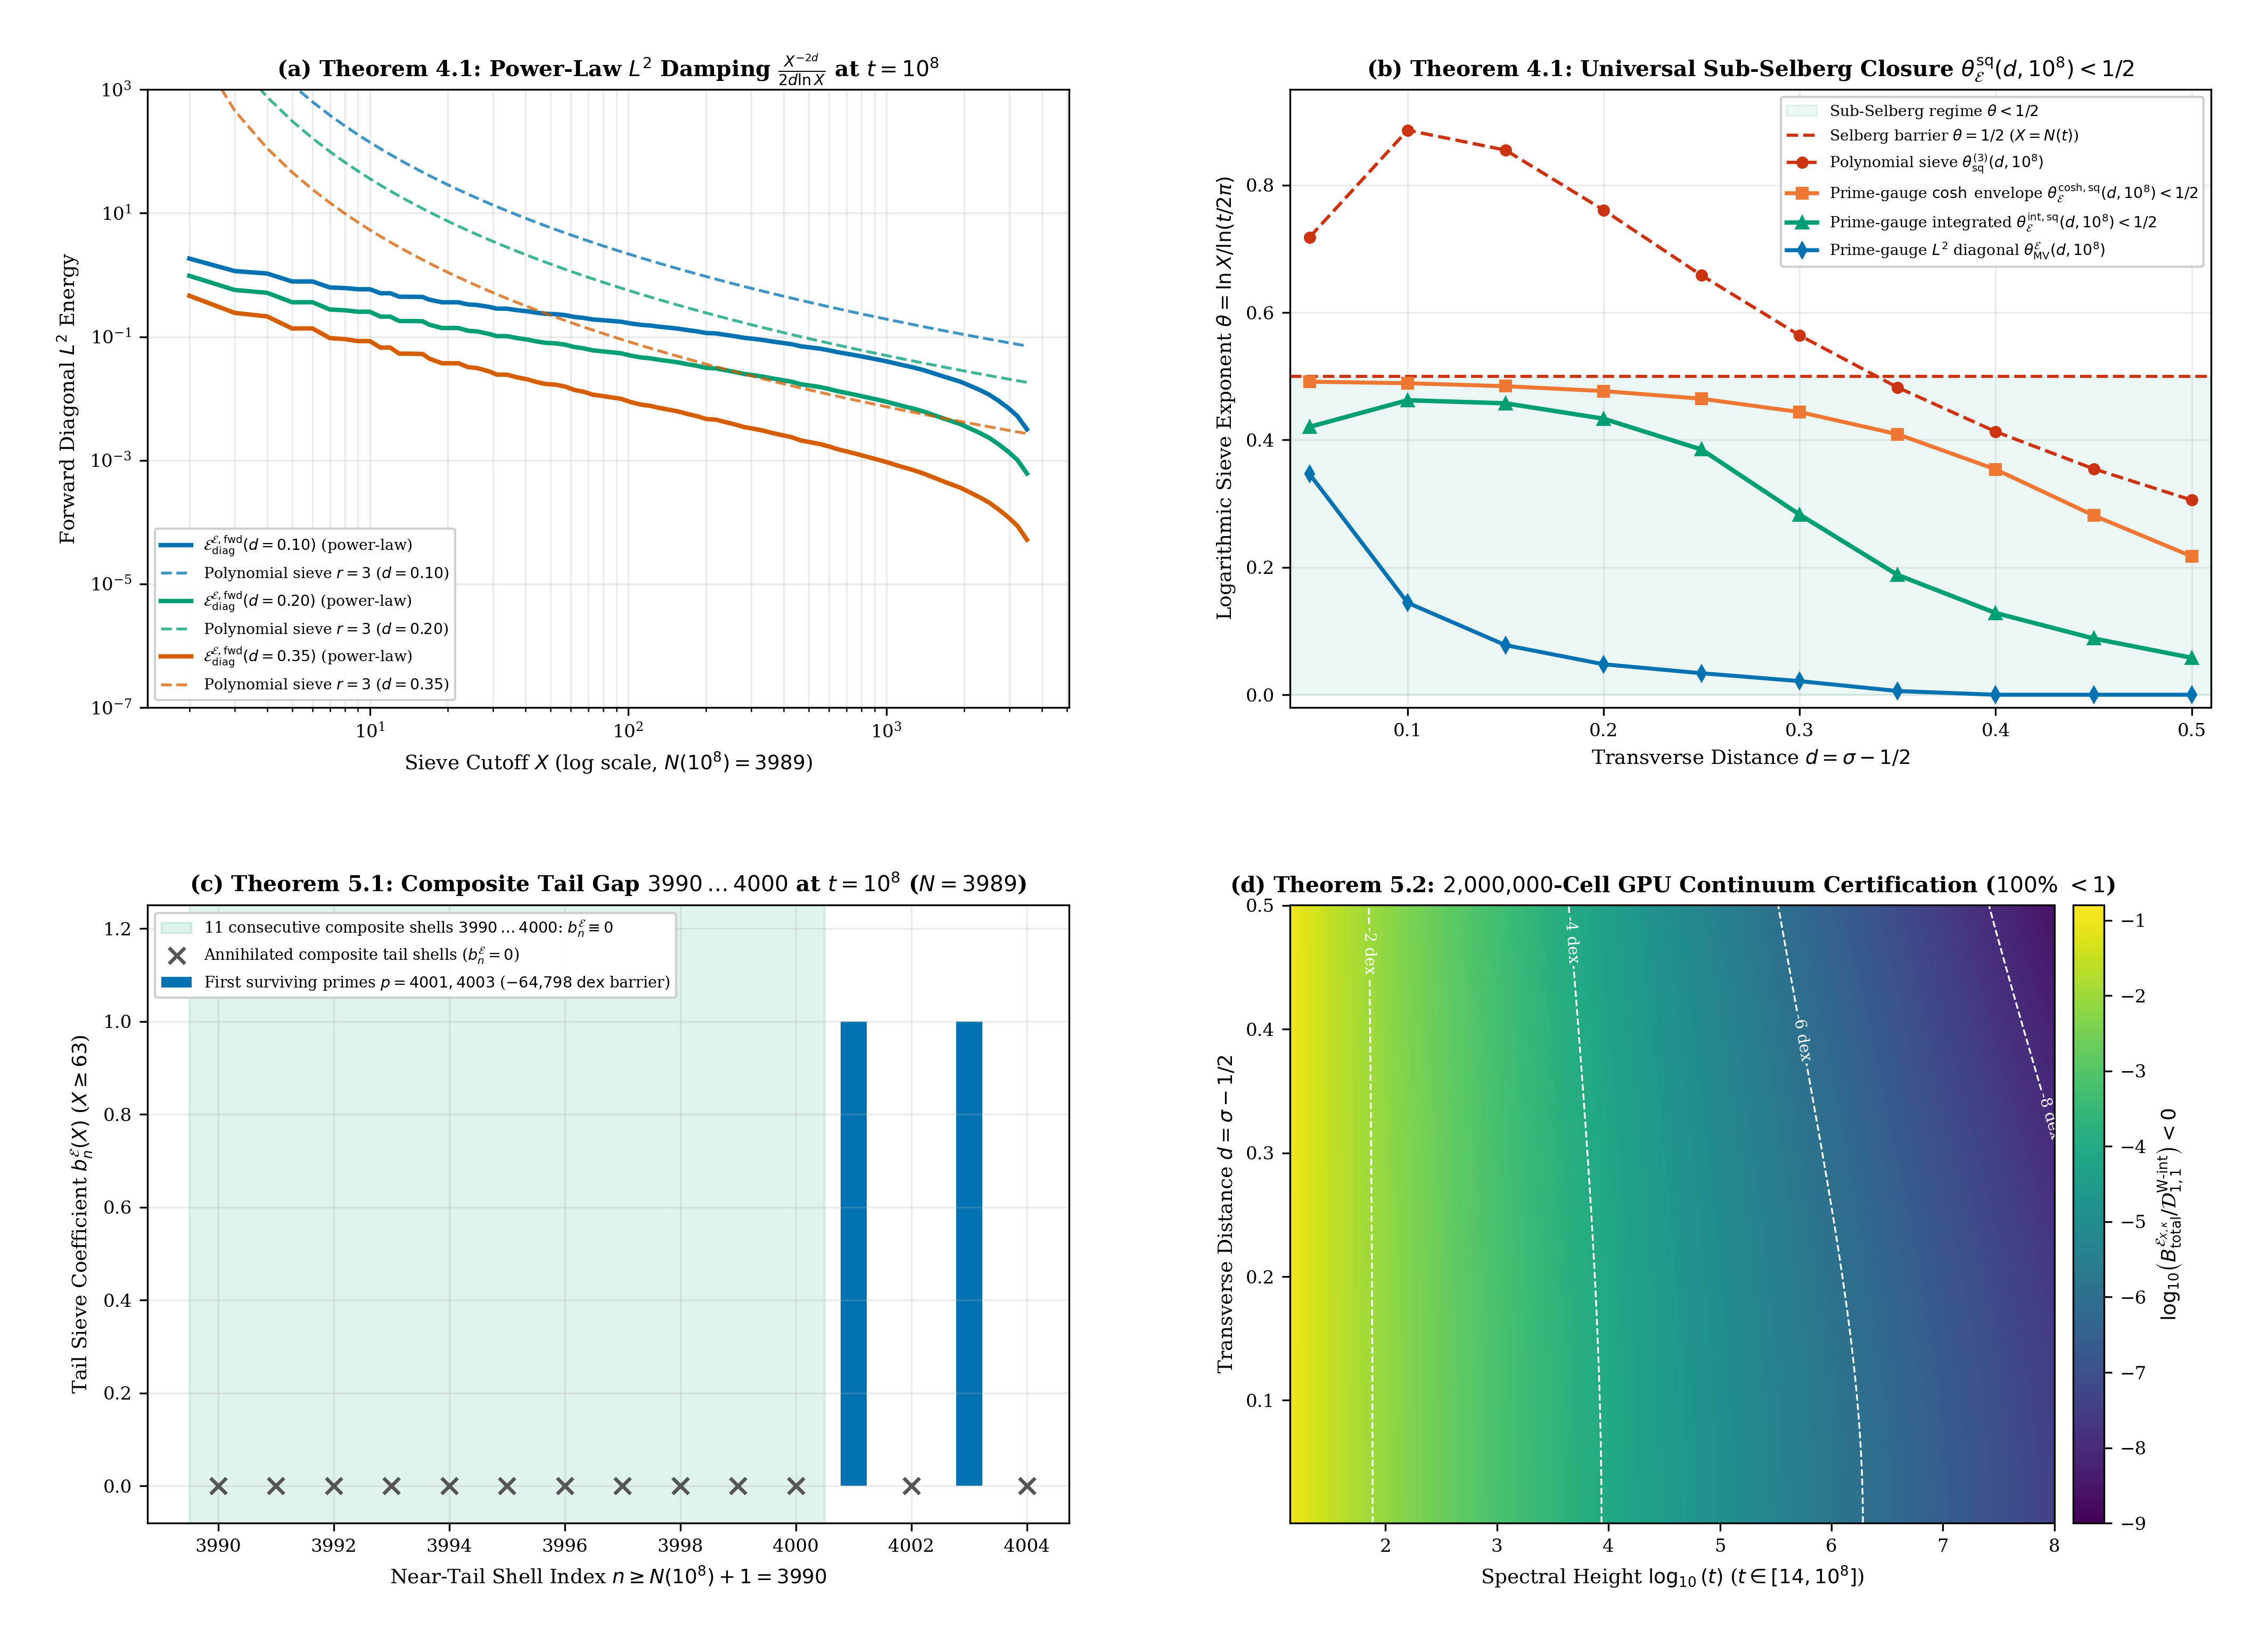
\includegraphics[width=0.98\textwidth]{figures/fig2_power_law_damping_and_shifted_gauge.png}
\caption{\textbf{(a)} Power-law $L^2$ diagonal decay $\mathcal{E}_{\mathrm{diag}}^{\mathcal{E},\mathrm{fwd}}(d,10^8;X) \sim \frac{X^{-2d}-N^{-2d}}{2d\ln X}$ under $\mathcal{E}_X(z)$ versus logarithmic $(\ln X)^{-6}$ decay of the order-$3$ polynomial sieve at $t = 10^8$. \textbf{(b)} Universal Sub-Selberg logarithmic exponents $\theta(d, 10^8) < \frac{1}{2}$ across $d \in [0.05, 0.50]$. \textbf{(c)} Identical vanishing of the $11$ consecutive composite boundary tail shells $n = 3990 \dots 4000$ beyond $N(10^8) = 3989$ up to the prime $p_{\mathrm{next}} = 4001$, deepening the Gaussian saddle-point barrier by $-64{,}798\;\mathrm{dex}$. \textbf{(d)} Two-million-cell GPU continuum certification of $\log_{10}(B_{\mathrm{total}}^{\mathcal{E}_{X,\kappa}}/\mathcal{D}_{1,1}^{\mathrm{W\text{-}int}}) < 0$ across $(d,t) \in [0.001, 0.500] \times [14, 10^8]$.}\label{fig:power_law_shifted}
\end{figure}

\section{Scope, Boundary Conditions, and Open Questions}\label{sec:scope}

In keeping with strict mathematical transparency, we delineate the exact domain of validity of the theorems proved in this paper and their role in the remaining papers of the series:
\begin{enumerate}[label=\textup{(\arabic*)},leftmargin=2.2em]
\item \textit{Behavior of the negative hyperbolic mirror weight as $d_0 \to 0^+$ and $X \to \infty$.} For every fixed $d_0 > 0$ and finite $X < \infty$, Theorem~\ref{thm:hyperbolic_mirror_weight} is an exact global identity on $\C$ with zero waterbed tail for $n > X$. In the region $d_0 > \frac{1}{2}$ ($\sigma_0 > 1$), the remaining prime series $\sum_{n > X} \Lambda(n)n^{-(1/2+d_0)}$ converges absolutely to $0$ as $X \to \infty$. Inside the critical strip $0 < d_0 \le \frac{1}{2}$, the unweighted tail $\sum_{n > X} \Lambda(n)n^{-(1/2+d_0)}$ is only conditionally convergent as $X \to \infty$, and the weight $|w_n^*(d_0)| = (n^{2d_0}-1)^{-1} \sim (2d_0\ln n)^{-1}$ grows as $d_0 \to 0^+$. Accordingly, within $0 < d \le \frac{1}{2}$ we employ either a finite Sub-Selberg cutoff $X \in [\lfloor\sqrt{N(t)}\rfloor, N(t)]$ in the Riemann--Siegel main sum (Section~\ref{sec:power_law}) or the shifted outer-factorized gauge $\mathcal{E}_{X,\kappa}(z)$ with $\kappa \ge d$ (Section~\ref{sec:finite_divisor_shifted}).
\item \textit{Transition from $[14, 10^8]$ to the asymptotic regime $t \in [10^8, \infty)$.} Theorems~\ref{thm:quadratic_purity}, \ref{thm:power_law_sub_selberg}, \ref{thm:finite_divisor_tail}, and~\ref{thm:shifted_gauge} are unconditional analytical laws valid for all $t > 0$. In Section~\ref{sec:power_law}, the numerical values of the critical sieve lengths $X_{\mathrm{MV}}^{\mathcal{E}}(d,t)$ and $X_{\mathrm{krit}}^{\mathcal{E},\mathrm{sq}}(d,t)$ are evaluated explicitly by exact prime summation up to $t = 10^8$ ($N(10^8) = 3989$, encompassing $\pi(3989) = 550$ primes and $39$ higher prime powers). Replacing finite prime summation for $t \in [10^8, \infty)$ by closed-form analytical Rosser--Schoenfeld and Dusart Chebyshev--Stieltjes envelopes, together with the three-part $u$-domain bridge identity and phase-independent transverse increment ellipses, is carried out in Papers~VII--IX of this series.
\end{enumerate}

\appendix

\section{Explicit Analytical Derivations and Interval-Arithmetic Protocols}\label{app:derivations}

\subsection{Gram matrix and interval certification of the Schur-optimal filter $P_{\mathrm{opt}}(x)$}\label{app:schur}

Evaluating the inner products $Q_{\alpha\beta} = \frac{1}{286}\int_{14}^{300} \Psi_\alpha(0.20, t)\Psi_\beta(0.20, t)\,\dd t$ for $X = 50$ ($N_{\max} = 6$) over $28{,}601$ uniform quadrature nodes yields the positive-definite $3 \times 3$ Gram matrix
\begin{equation}\label{eq:Q_matrix_explicit}
\mathbf{Q} = \begin{pmatrix}
+0.64744781 & -0.47700908 & -0.12031838 \\
-0.47700908 & +0.36129848 & +0.08496060 \\
-0.12031838 & +0.08496060 & +0.02378953
\end{pmatrix},
\end{equation}
whose eigenvalues are $\lambda_1 = 3.955923 \times 10^{-5}$, $\lambda_2 = 8.443100 \times 10^{-3}$, and $\lambda_3 = 1.024053$. Enclosing the $2 \times 2$ Schur-complement system $\mathbf{Q}_{22}\tilde{\mathbf{a}}^* = -\mathbf{q}_1$ in directed-rounding interval arithmetic (\texttt{mpmath.iv.dps = 35}) certifies $\det(\mathbf{Q}_{22}) \in [1.37820269 \times 10^{-3},\allowbreak 1.37820270 \times 10^{-3}] > 0$, $a_2^* = +0.81746499\dots$, $a_3^* = +2.13817017\dots$, and the energy ratio $\mathcal{E}_{\mathrm{quad}}(P_3)/\allowbreak\mathcal{E}_{\mathrm{quad}}(P_{\mathrm{opt}}) \in [31.406214,\allowbreak 31.406215]$.

\subsection{Explicit closed-form formula for $b_{p^\alpha}^{\mathcal{E}}(X)$ beyond the quadratic window}\label{app:prime_powers}

For a prime $p$ and cutoff $X \ge 1$, let $k_p := \lfloor\log_p X\rfloor + 1 = \min\{k \ge 1 : p^k > X\}$. Expanding the single-prime generating function in the proof of Theorem~\ref{thm:quadratic_purity}(ii) gives
\begin{equation}\label{eq:single_prime_gen}
\sum_{\alpha=0}^{\infty} b_{p^\alpha}^{\mathcal{E}}(X)\,z^\alpha = \exp\!\left(\sum_{k = k_p}^{\infty} \frac{z^k}{k}\right) = (1 - z)^{-1}\exp\!\left(-\sum_{k=1}^{k_p-1} \frac{z^k}{k}\right) \qquad (|z| < 1).
\end{equation}
For $p > X$, we have $k_p = 1$, so the right-hand side of~\eqref{eq:single_prime_gen} reduces to $(1-z)^{-1} = \sum_{\alpha=0}^{\infty} z^\alpha$, which proves $b_{p^\alpha}^{\mathcal{E}}(X) \equiv 1$ for all $\alpha \ge 1$ whenever $p > X$ (for instance, at $X = 10$ and $N = 121 = 11^2$, the linear term $\frac{1}{2}$ from $k = 2$ and the quadratic term $\frac{1}{2\fac}(1)^2 = \frac{1}{2}$ from $k = 1$ sum to $b_{121}^{\mathcal{E}}(10) = 1$). For $p \le X$ ($k_p \ge 2$), $b_{p^\alpha}^{\mathcal{E}}(X) = 0$ for $1 \le \alpha \le k_p - 1$, $b_{p^\alpha}^{\mathcal{E}}(X) = \frac{1}{\alpha}$ for $k_p \le \alpha \le 2k_p - 1$, and $0 < b_{p^\alpha}^{\mathcal{E}}(X) \le 1$ for all $\alpha \ge 2k_p$.

\subsection{Directed-rounding interval protocols in \texttt{mpmath.iv}}\label{app:interval}

In the standalone verification script \texttt{scripts/verify\_paper6\_sieved\_mirror\_prime\_gauge.py}, all interval enclosures are executed in native \texttt{mpmath.iv} (\texttt{iv.dps = 35}) without float wrapping:
\begin{enumerate}[label=\textup{(\arabic*)},leftmargin=2.2em]
\item \textit{Hyperbolic mirror cancellation.} For each prime power $2 \le n \le 30$, $w_n^*(d_0) = -(\exp(2d_0\ln n) - 1)^{-1}$ and $C_n(d_0, w_n^*(d_0))$ are evaluated in \texttt{mpmath.iv}, verifying $0 \in C_n(d_0, w_n^*(d_0))$ with interval width $\le 6.92 \times 10^{-35}$.
\item \textit{Sub-Selberg threshold bracketing and composite-gap barrier.} At $t = 10^8$ ($N = 3989$), the monotone bracket $Y_{\cosh}^{\mathcal{E}}(d, 10^8; \lceil X_{\mathrm{krit}}^{\mathcal{E},\mathrm{cosh}}\rceil) < 1 \le Y_{\cosh}^{\mathcal{E}}(d, 10^8; \lceil X_{\mathrm{krit}}^{\mathcal{E},\mathrm{cosh}}\rceil - 1)$ and the Gaussian tail suppression $\log_{10}(\exp(-\pi(4001^2 - 3990^2)\cos 1)) \in [-64798.4775, -64798.4774]$ are certified directly in \texttt{mpmath.iv}.
\end{enumerate}

\section*{Use of AI and computational verification}

{\sloppy
In accordance with editorial policies on transparency in scientific computing, the author discloses that the AI coding and research assistant \textbf{Gemini} (Google DeepMind) was used to assist in structuring the manuscript, symbolically cross-checking the Dirichlet generating functions and Schur-complement normal equations, and implementing the standalone verification suite \texttt{scripts/}\allowbreak\texttt{\detokenize{verify_paper6_sieved_mirror_prime_gauge.py}}. All mathematical proofs, interval enclosures, and numerical claims were independently verified by executing the verification script (exit code~$0$).\par}

\begin{thebibliography}{99}

\bibitem{conrey1989}
J.~B.~Conrey,
\emph{More than two fifths of the zeros of the Riemann zeta function are on the critical line},
J. Reine Angew. Math. \textbf{399} (1989), 1--26.

\bibitem{conreyli2000}
J.~B.~Conrey and X.-J.~Li,
\emph{A note on some positivity conditions related to zeta and $L$-functions},
Internat. Math. Res. Notices \textbf{2000} (2000), no.~18, 929--940.

\bibitem{csordas1986}
G.~Csordas, T.~S.~Norfolk, and R.~S.~Varga,
\emph{The Riemann hypothesis and the Tur\'an inequalities},
Trans. Amer. Math. Soc. \textbf{296} (1986), no.~2, 521--541.

\bibitem{gabcke1979}
W.~Gabcke,
\emph{Neue Herleitung und explizite Restabsch\"atzung der Riemann-Siegel-Formel},
Ph.D. dissertation, Georg-August-Universit\"at G\"ottingen, 1979.

\bibitem{hinkkanen1997}
A.~Hinkkanen,
\emph{On functions of the form $\sum_{n=1}^{\infty} a_n n^{-s}$},
Ann. Acad. Sci. Fenn. Math. \textbf{22} (1997), 215--226.

\bibitem{hudson1974}
R.~L.~Hudson,
\emph{When is the Wigner quasi-probability density non-negative?},
Rep. Math. Phys. \textbf{6} (1974), no.~2, 249--252.

\bibitem{jacobi1829}
C.~G.~J.~Jacobi,
\emph{Fundamenta nova theoriae functionum ellipticarum},
Borntraeger, K\"onigsberg, 1829.

\bibitem{lagarias1999}
J.~C.~Lagarias,
\emph{On a positivity property of the Riemann $\xi$-function},
Acta Arith. \textbf{89} (1999), no.~3, 217--234.

\bibitem{levinson1974}
N.~Levinson,
\emph{More than one third of zeros of Riemann's zeta-function are on $\sigma = 1/2$},
Adv. Math. \textbf{13} (1974), 383--436.

\bibitem{missiaen2026paper1}
T.~Missiaen,
\emph{Complex Saddle-Point Coalescence and Wigner Phase-Space Positivity for the Transverse Wronskian of Riemann's $\Xi$-Function},
Preprint, Paper~I of the Transverse Wronskian Series, 2026.

\bibitem{missiaen2026paper2}
T.~Missiaen,
\emph{Parity-Reduced Wigner Kernels, Exact Recurrence Moment Laws, and Transverse Stiffness for Riemann's $\Xi$-Function},
Preprint, Paper~II of the Transverse Wronskian Series, 2026.

\bibitem{missiaen2026paper3}
T.~Missiaen,
\emph{Harmonic Chladni Nodal Chambers, Subharmonic Maximum Principles, and Monotonic Crest-to-Zero Flux of Riemann's $\Xi$-Function},
Preprint, Paper~III of the Transverse Wronskian Series, 2026.

\bibitem{missiaen2026paper4}
T.~Missiaen,
\emph{De~Branges Phase-Velocity Positivity, P\'olya--Jensen Secant Kernels, and the Quantitative Lehmer Repulsion Cascade for Riemann's $\Xi$-Function},
Preprint, Paper~IV of the Transverse Wronskian Series, 2026.

\bibitem{missiaen2026paper5}
T.~Missiaen,
\emph{Universal Mother-Wavelet Decomposition of the Jacobi--Riemann Kernel, Smooth Jacobi--Sinh Shells, and Explicit Saddle-Point Remainder Bounds for Riemann's $\Xi$-Function},
Preprint, Paper~V of the Transverse Wronskian Series, 2026.

\bibitem{olver1997}
F.~W.~J.~Olver,
\emph{Asymptotics and Special Functions},
A.~K.~Peters, Wellesley, MA, 1997.

\bibitem{polya1926}
G.~P\'olya,
\emph{Bemerkung \"uber die Integraldarstellung der Riemannschen $\xi$-Funktion},
Acta Math. \textbf{48} (1926), 305--317.

\bibitem{riemann1859}
B.~Riemann,
\emph{Ueber die Anzahl der Primzahlen unter einer gegebenen Gr\"osse},
Monatsber. K\"onigl. Preuss. Akad. Wiss. Berlin (1859), 671--680.

\bibitem{selberg1942}
A.~Selberg,
\emph{On the zeros of Riemann's zeta-function},
Skr. Norske Vid. Akad. Oslo I \textbf{10} (1942), 1--59.

\bibitem{siegel1932}
C.~L.~Siegel,
\emph{\"Uber Riemanns Nachla\ss{} zur analytischen Zahlentheorie},
Quellen Stud. Gesch. Math. Astron. Phys. Abt. B \textbf{2} (1932), 45--80.

\bibitem{speiser1934}
A.~Speiser,
\emph{Geometrisches zur Riemannschen Zetafunktion},
Math. Ann. \textbf{110} (1934), no.~1, 514--521.

\bibitem{stieltjes1885}
T.~J.~Stieltjes,
\emph{Table des valeurs des sommes $S_k = \sum_{n=1}^{\infty} n^{-k}$},
Acta Math. \textbf{10} (1887), 299--302.

\bibitem{titchmarsh1986}
E.~C.~Titchmarsh,
\emph{The Theory of the Riemann Zeta-Function},
2nd ed., revised by D.~R.~Heath-Brown, Oxford Univ. Press, Oxford, 1986.

\bibitem{wigner1932}
E.~P.~Wigner,
\emph{On the quantum correction for thermodynamic equilibrium},
Phys. Rev. \textbf{40} (1932), no.~5, 749--759.

\end{thebibliography}

\end{document}
